\documentclass[12pt]{scrartcl}

\usepackage[utf8]{inputenc}
\usepackage{fontenc}
\usepackage[ngerman]{babel}

\usepackage{graphicx}
\usepackage{enumitem}
\usepackage{booktabs}
\usepackage{geometry}

\geometry{margin={15mm, 25mm, 15mm, 0}}

\usepackage{comment}
\usepackage[center]{caption}
\usepackage{caption}
\captionsetup{
	figurename=Fig.
}
\usepackage{marvosym}

\pagenumbering{arabic}
\usepackage{pst-blur}
\usepackage{pdfpages}
\usepackage{amsmath}
\usepackage{amssymb}

\usepackage{amsthm}
\usepackage[
colorlinks=true,
urlcolor=black,
linkcolor=black
]{hyperref}
\usepackage[locale=DE,per-mode=fraction]{siunitx}

\usepackage{multirow}

\usepackage{microtype}
\usepackage{parskip}


\usepackage{tikz}



\usepackage{enumitem}
\usepackage{acronym}
\usepackage{placeins}
\usepackage{fancyhdr}


\usepackage{multicol}
\usepackage{listings}



\begin{document}
	\pagestyle{fancy}
	\fancyhead[l]{RPTU Kaiserslautern-Landau\hfill Kryptographie\hfill Moritz Groh}
	\fancyfoot[c]{Das Design basiert auf den Designs von \textsc{Tommy Hofmann} und \href{https://www.instructables.com/Poly-Alphabetic-Cipher-Machine/}{\textcolor{blue}{twzoom}}.}
	
	\fontsize{24}{30}\selectfont
	
	\begin{center}
		\textbf{Bauanleitung für eine Lego-Engima}
		\vspace{1em}
	
	\end{center}
	\normalsize
	
	\textsc{Der Hebel:}
	\begin{figure}[h!]
		\centering
		\psframebox[blur=true,shadow=true]{
			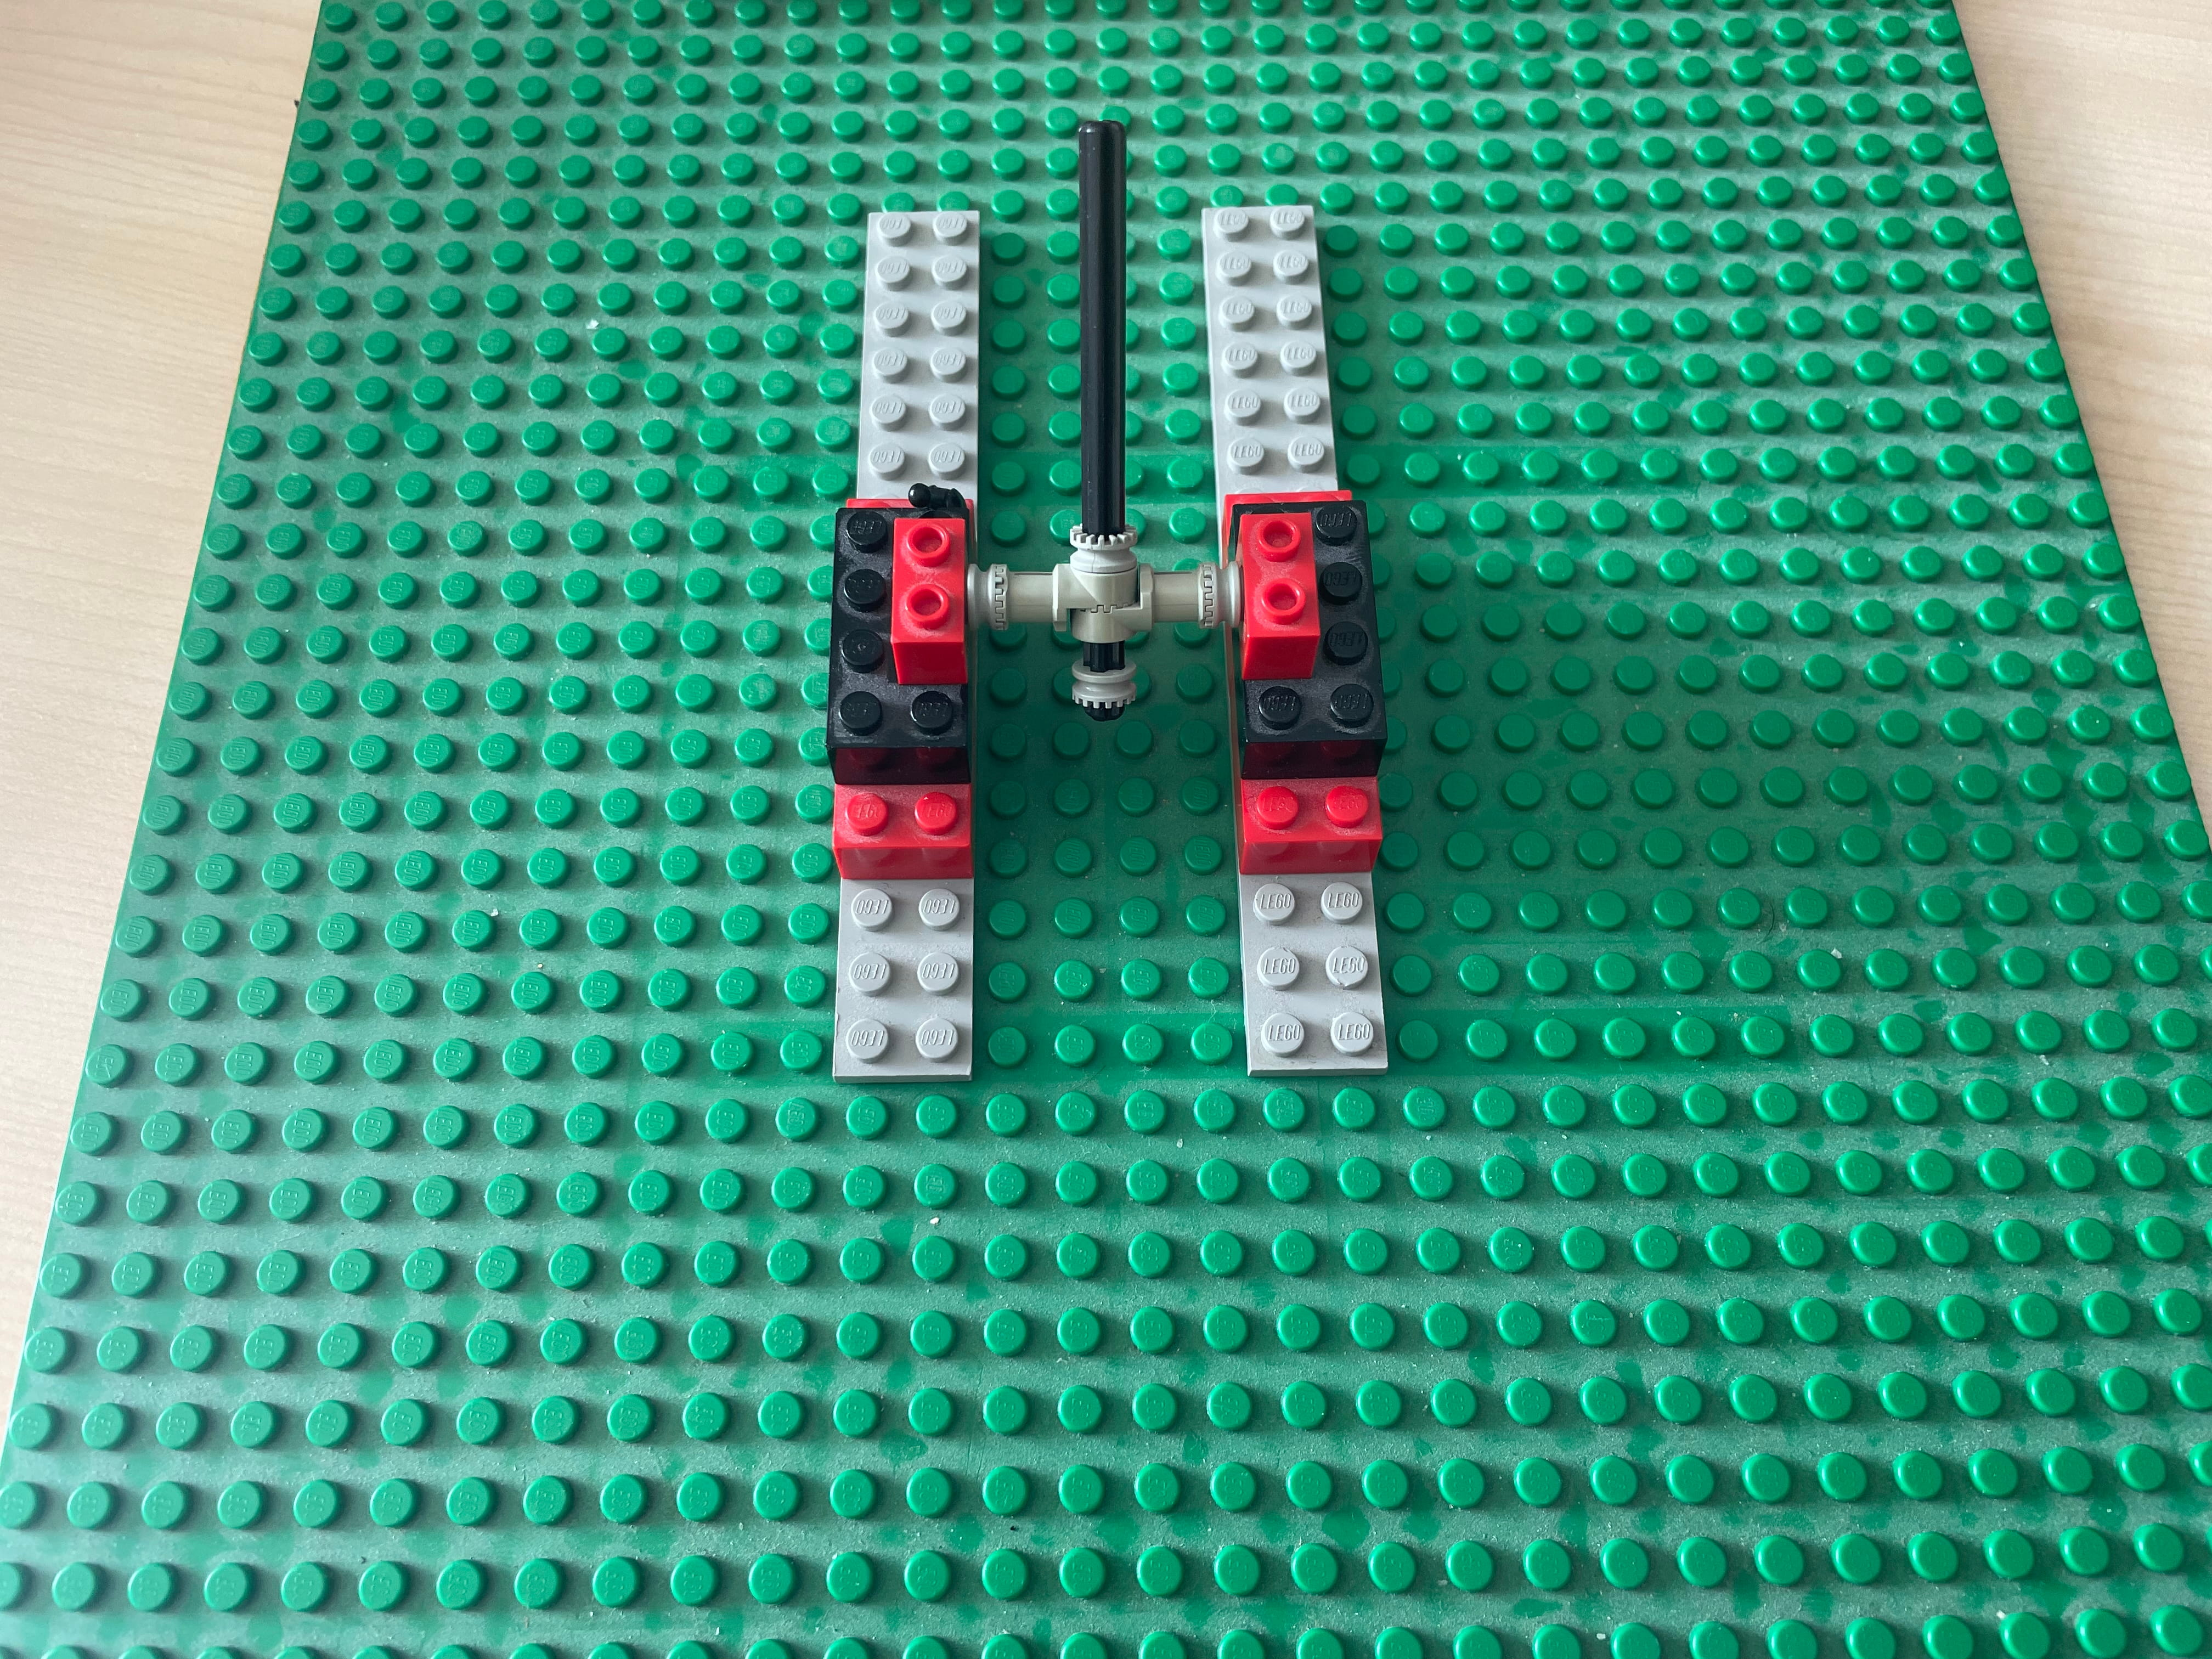
\includegraphics[width=200pt]{./Bilder/Hebel.jpg}}
	\end{figure}
	
	\textsc{Die Schiene:}
	
	\begin{minipage}{.5\textwidth}
		\centering
		\psframebox[blur=true,shadow=true]{
			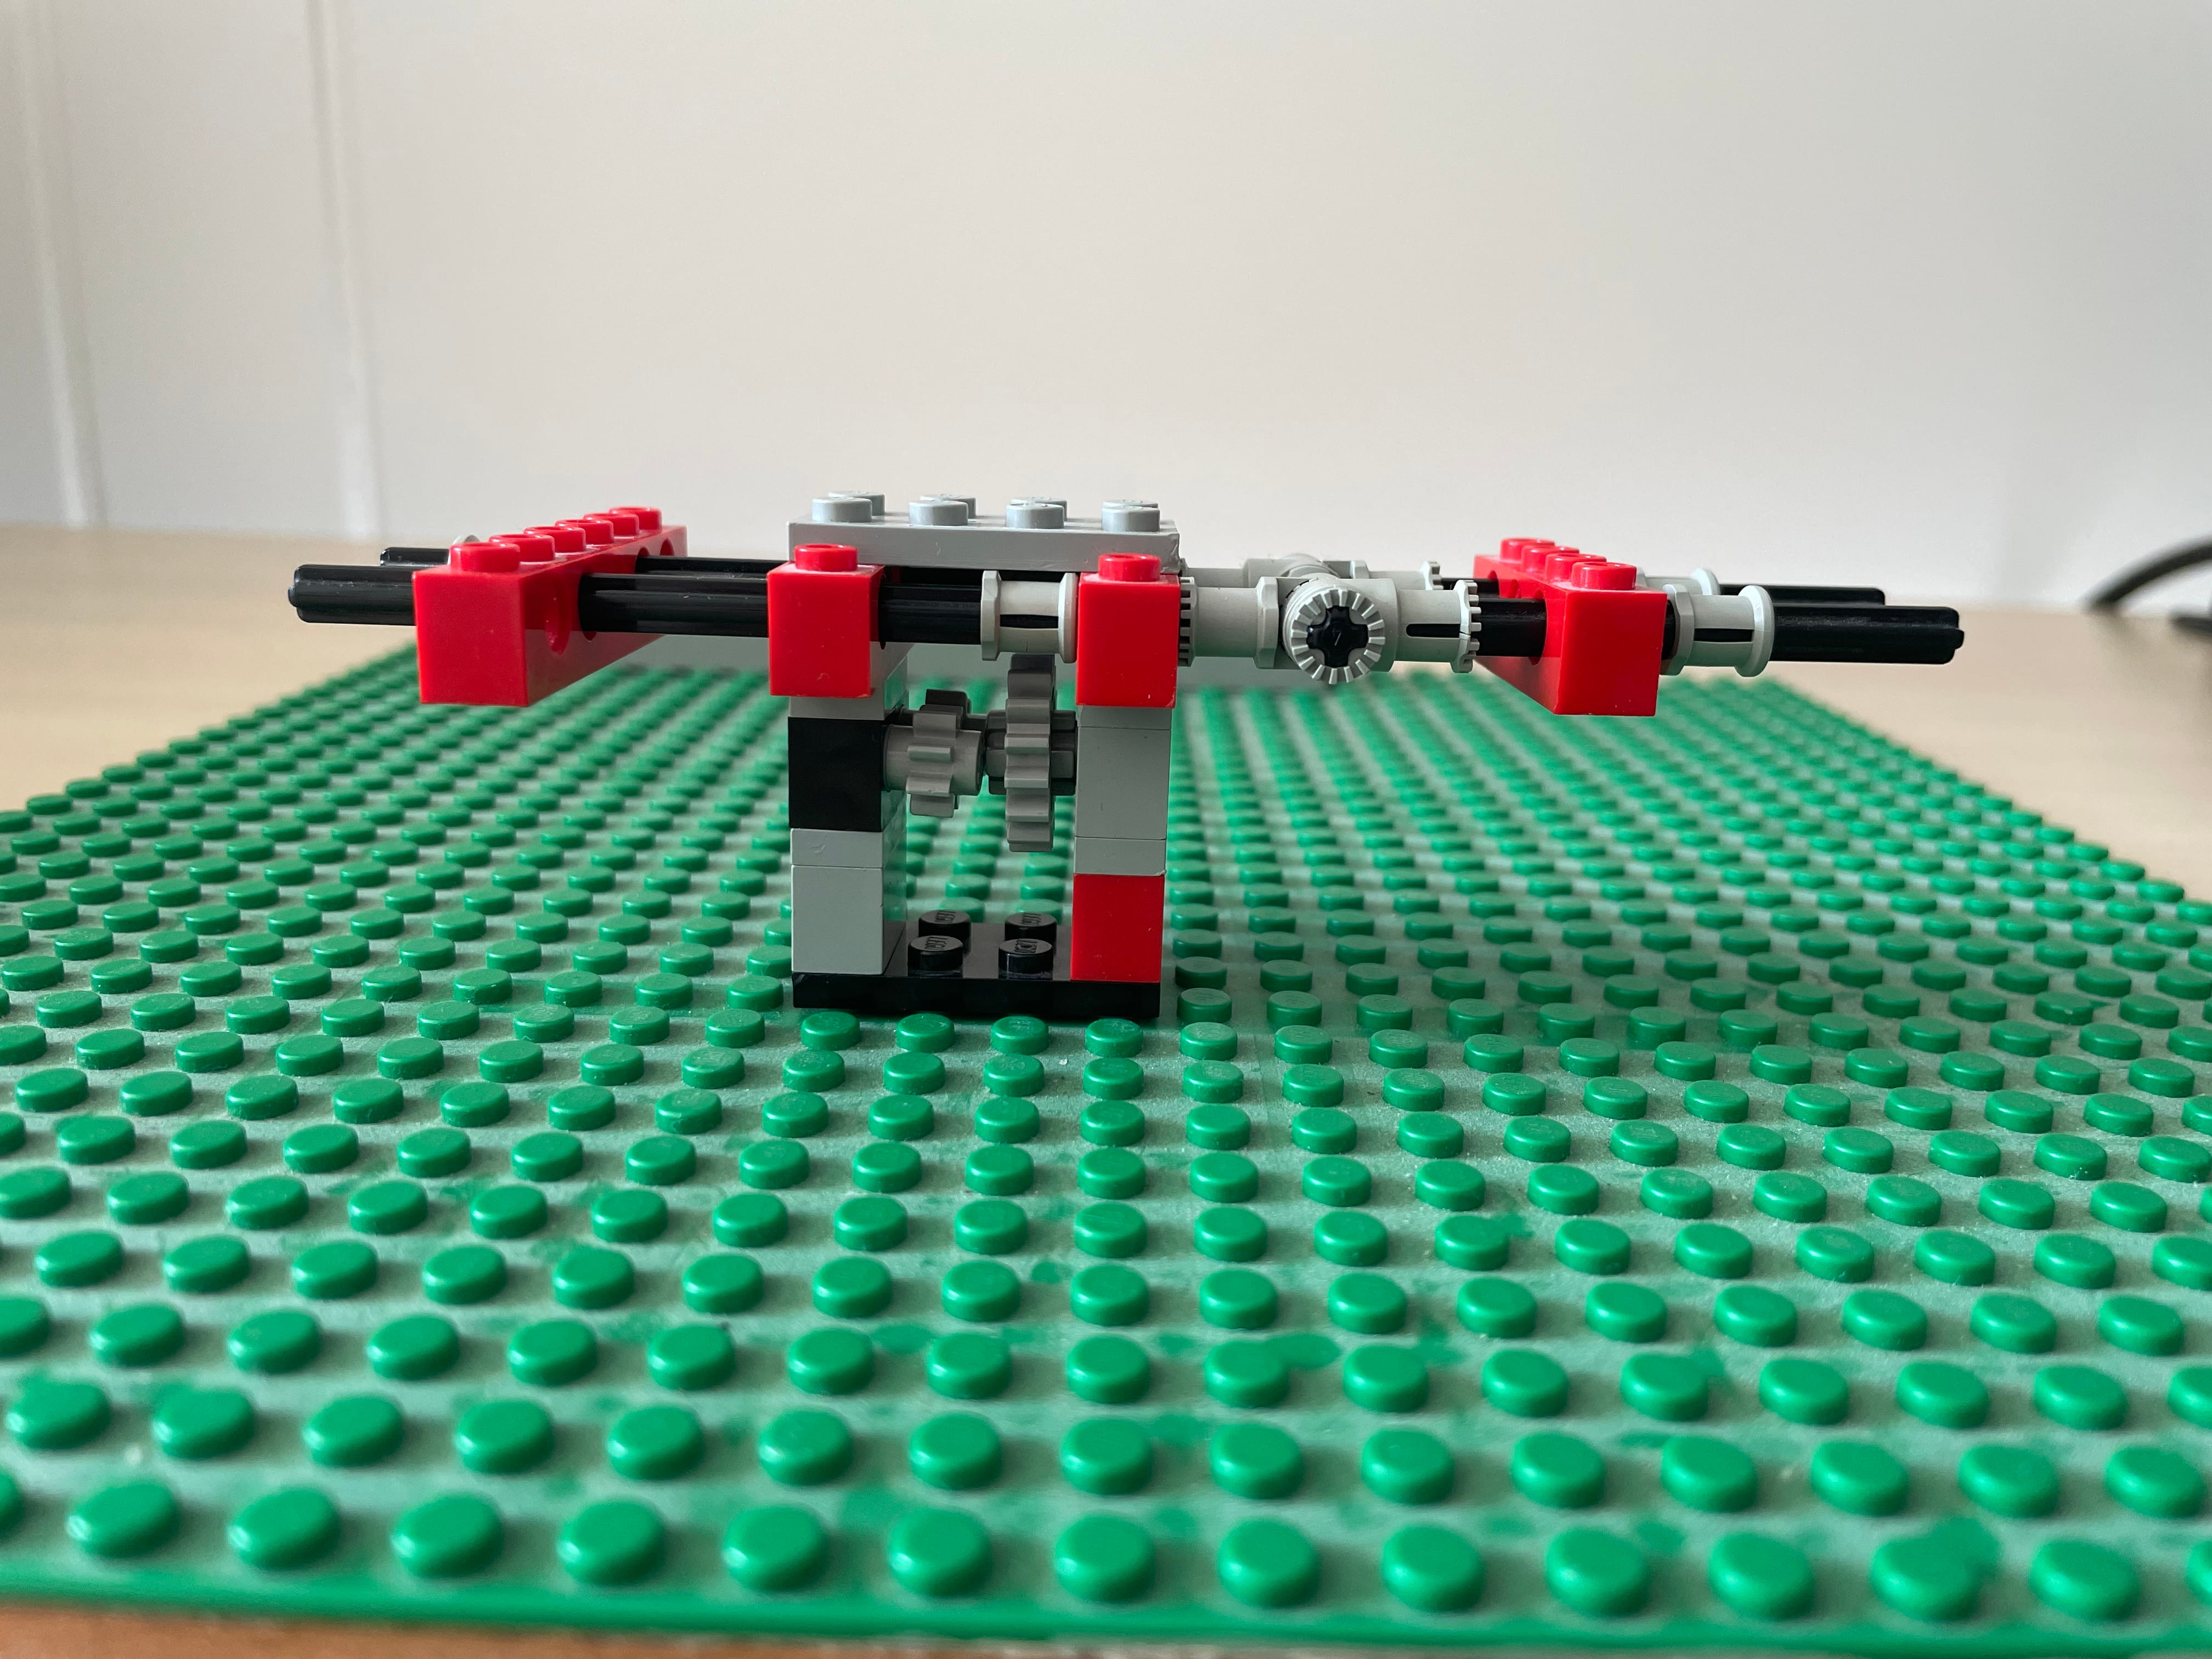
\includegraphics[width=200pt]{./Bilder/Zweirad_l.jpg}}
	\end{minipage}
	\begin{minipage}{.5\textwidth}
		\centering
		\psframebox[blur=true,shadow=true]{
			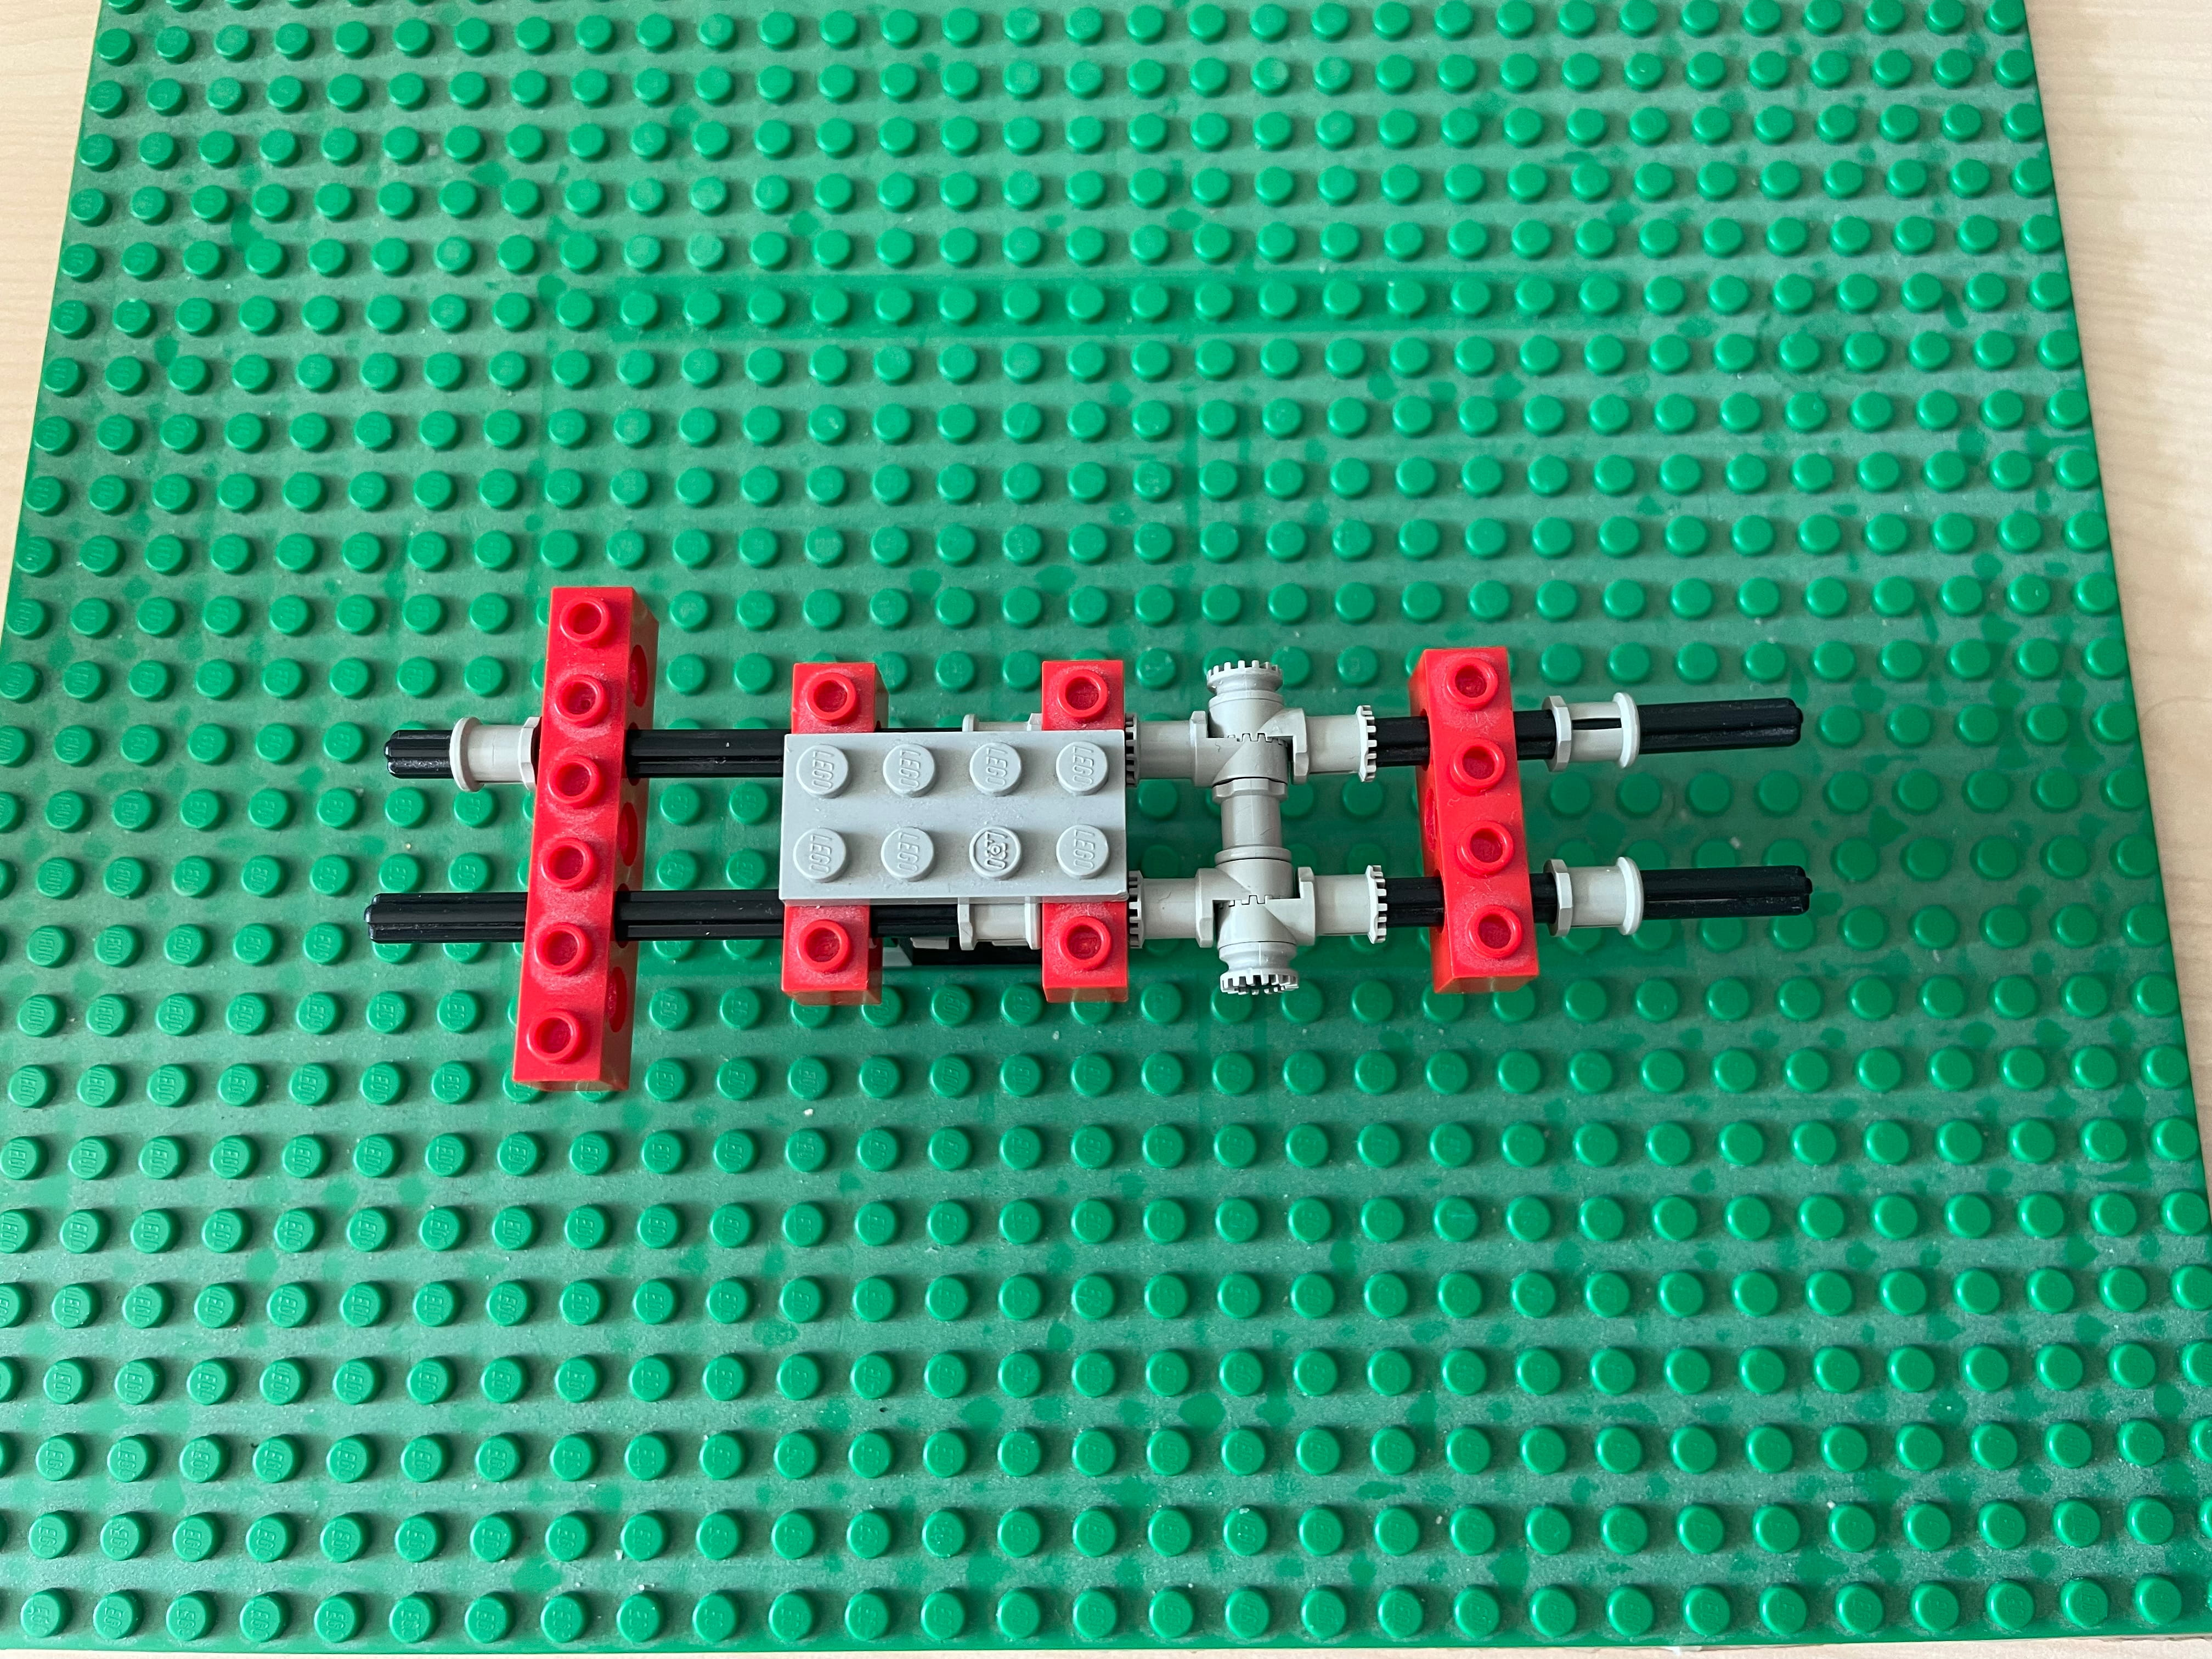
\includegraphics[width=200pt]{./Bilder/Zweirad_o.jpg}}
	\end{minipage}
	
	\begin{minipage}{.5\textwidth}
		\centering
		\psframebox[blur=true,shadow=true]{
			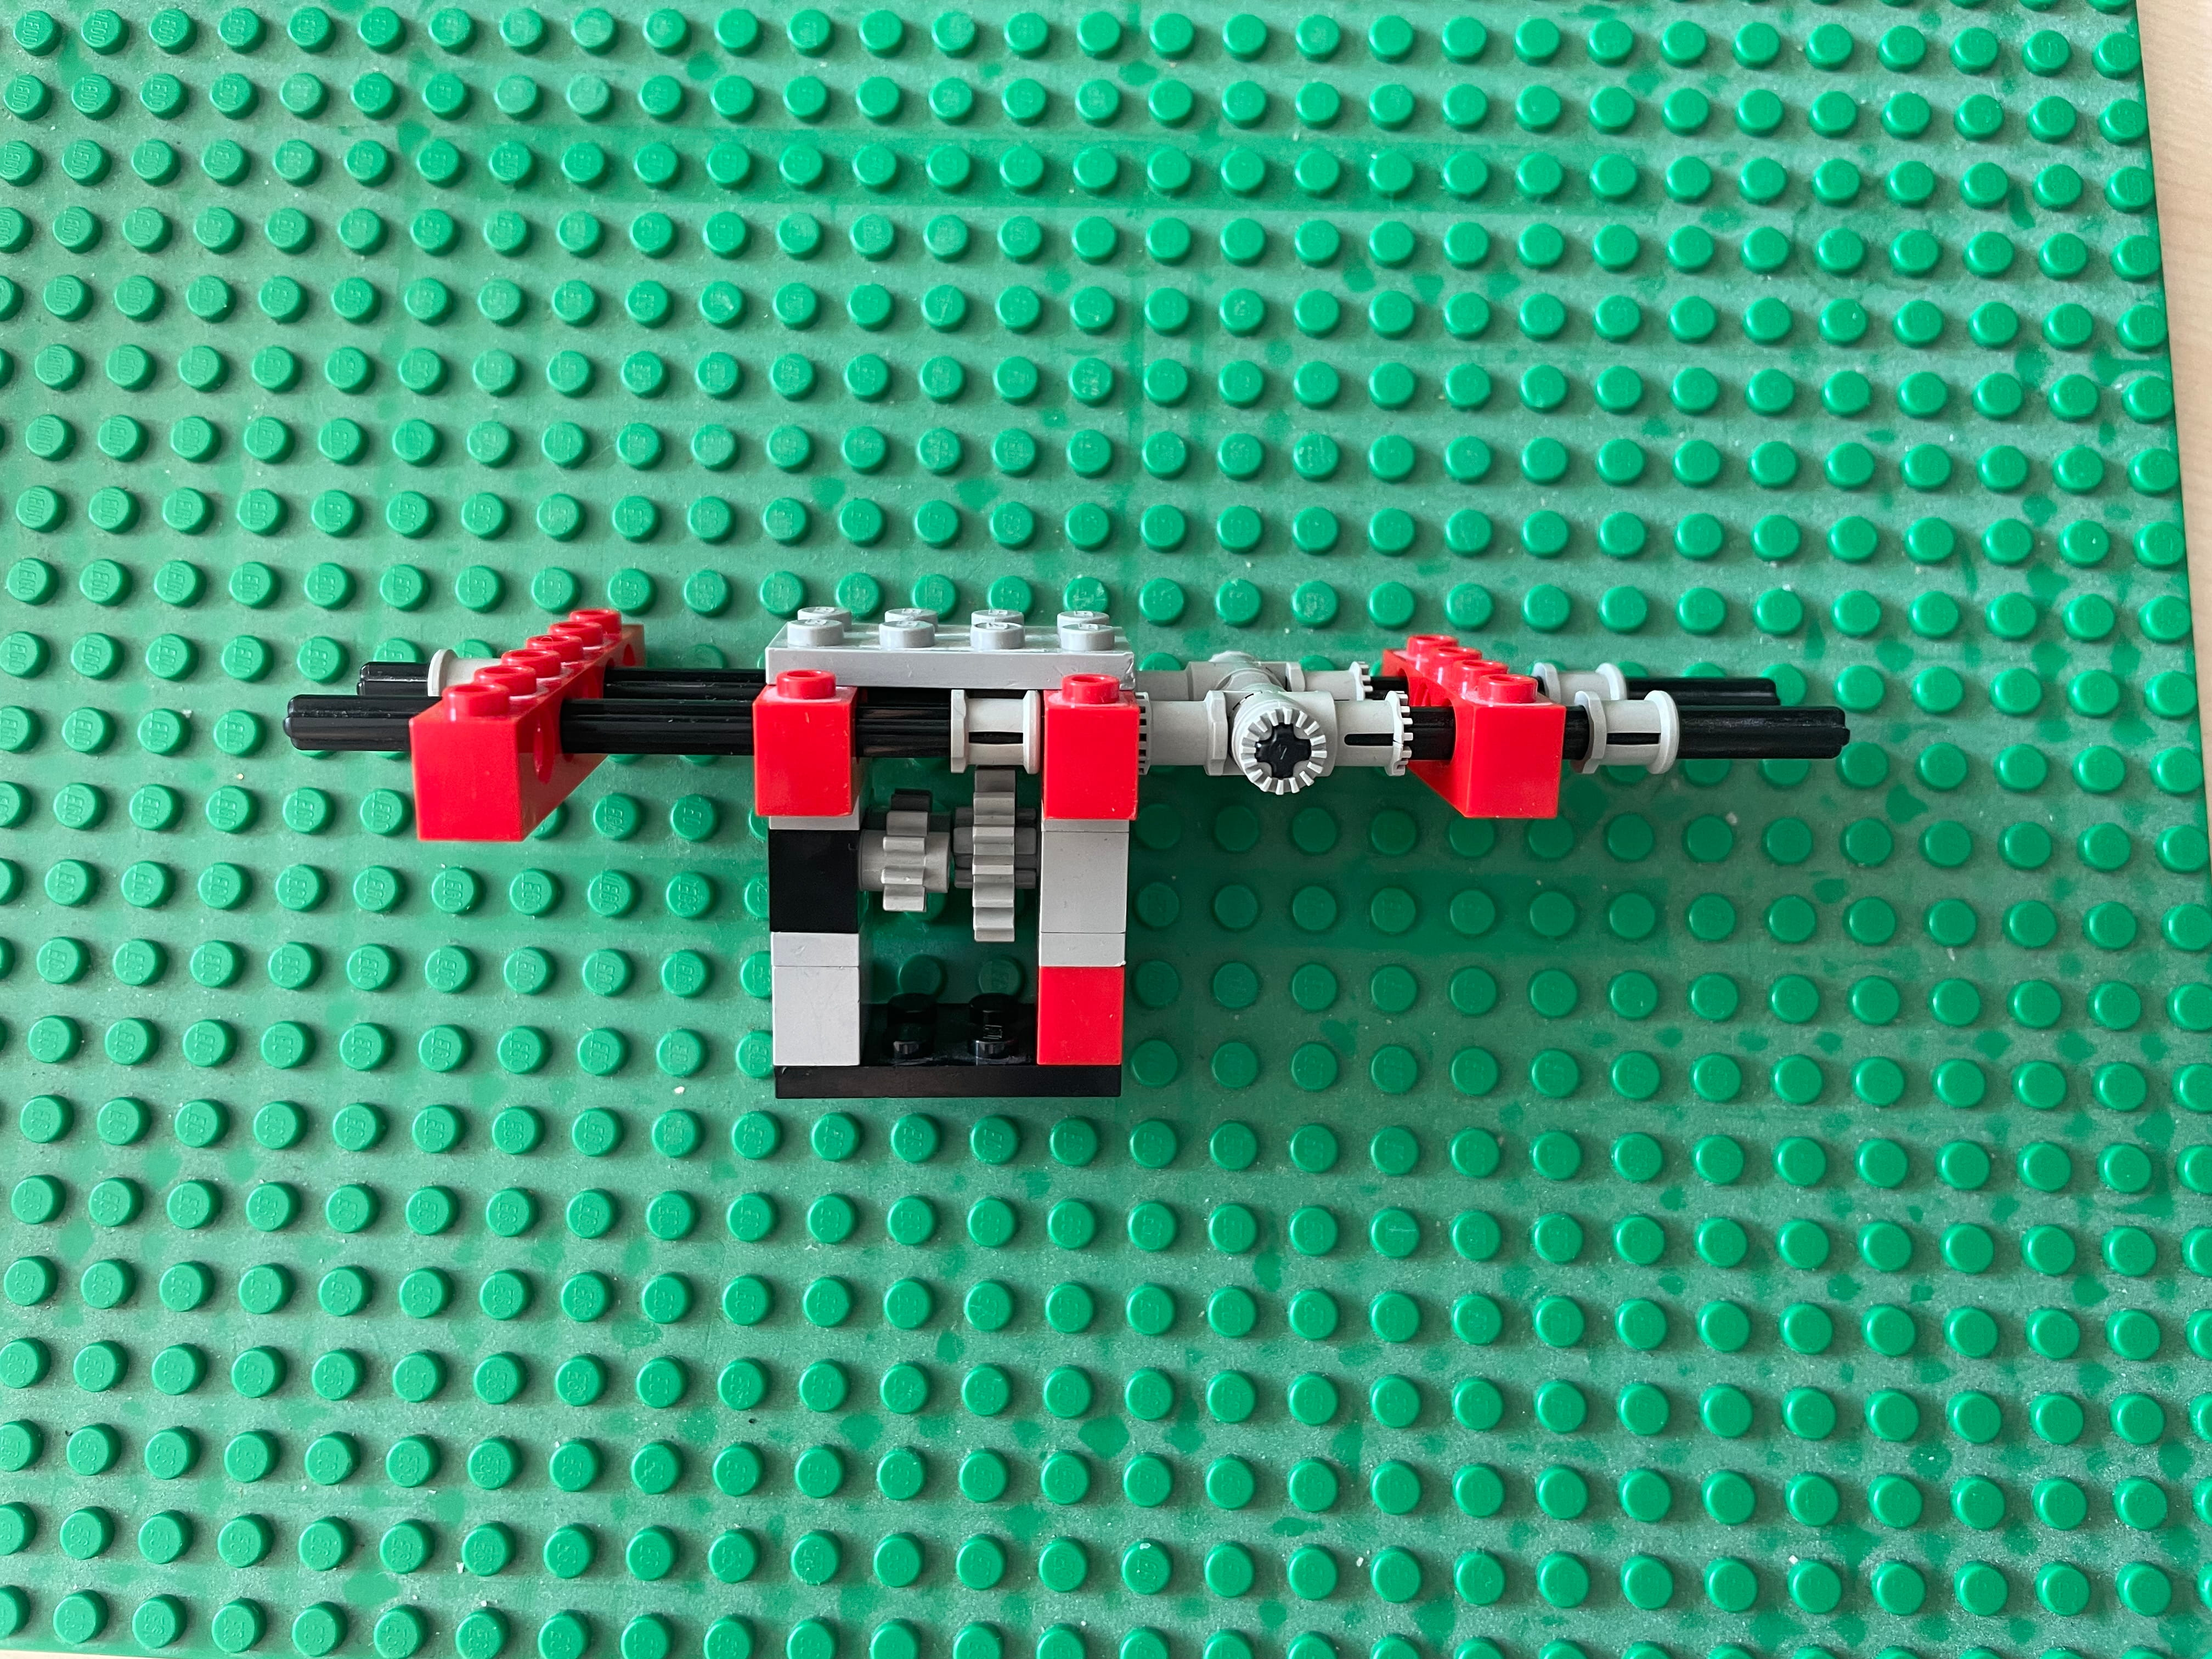
\includegraphics[width=200pt]{./Bilder/Zweirad_ls.jpg}}
	\end{minipage}
	\begin{minipage}{.5\textwidth}
		\centering
		\psframebox[blur=true,shadow=true]{
			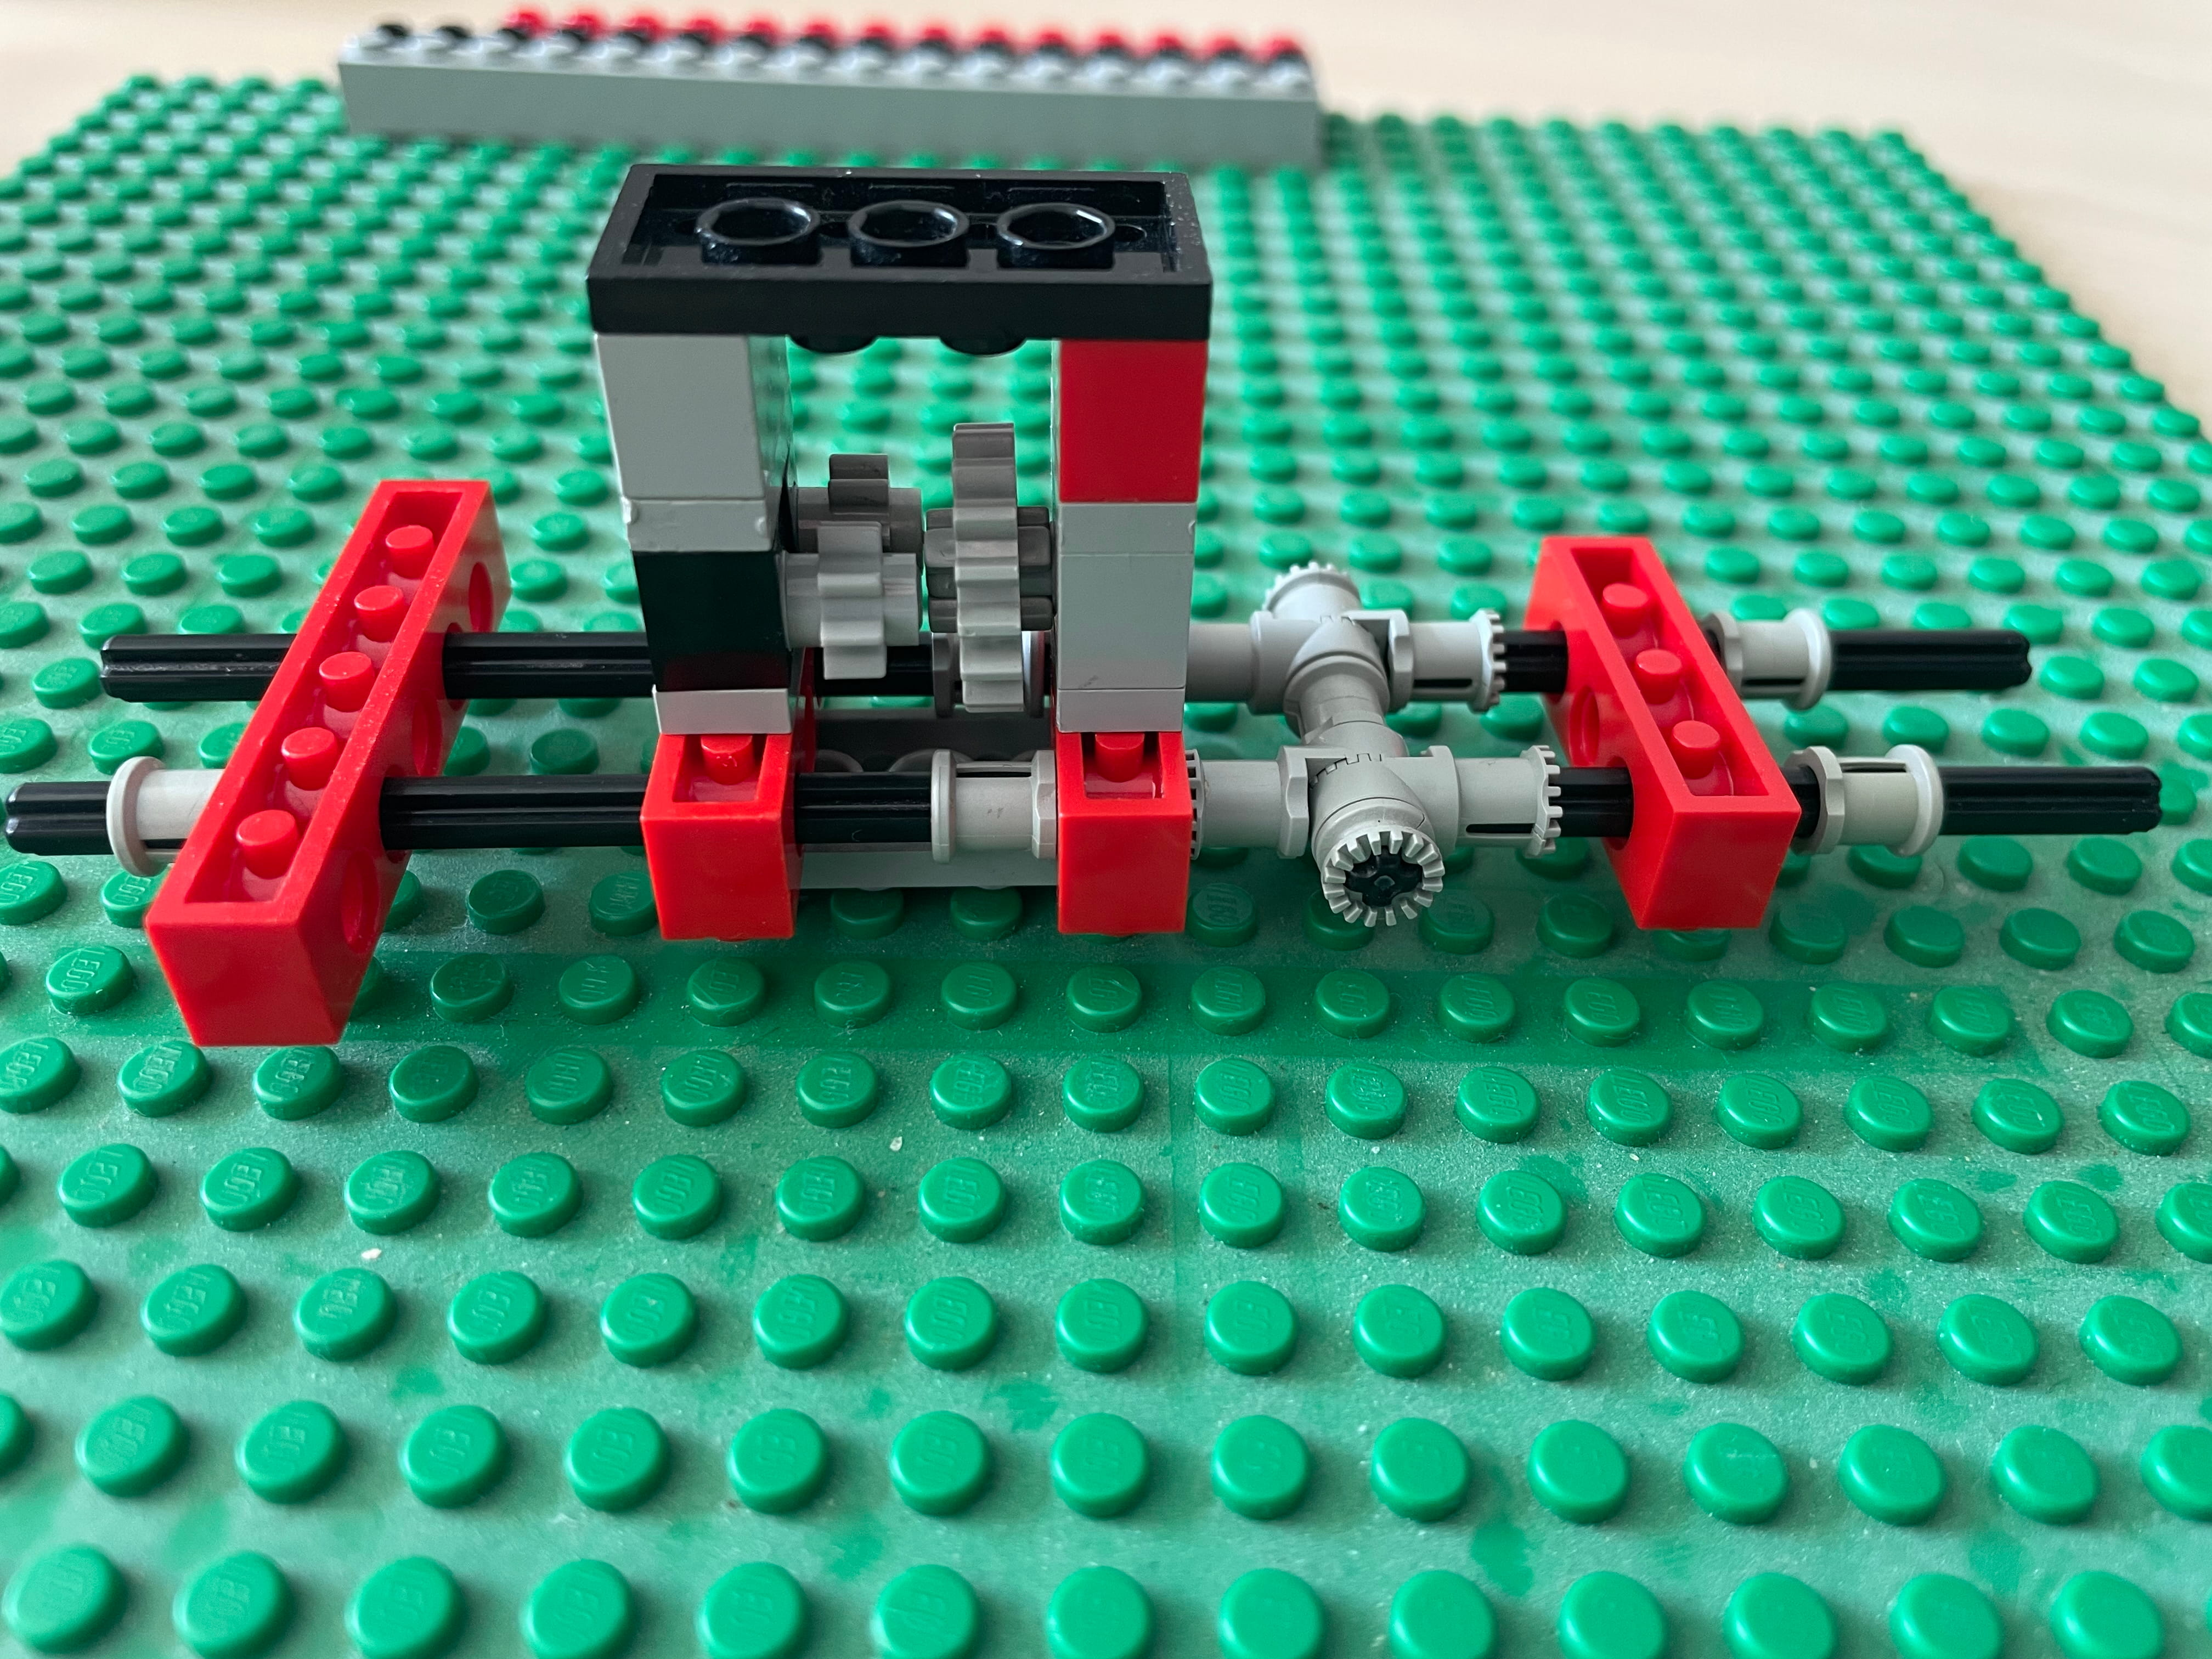
\includegraphics[width=200pt]{./Bilder/Zweirad_verk.jpg}}
	\end{minipage}
	\newpage
	\textsc{Das Gestell:}
	
	\begin{minipage}{.5\textwidth}
		\centering
		\psframebox[blur=true,shadow=true]{
			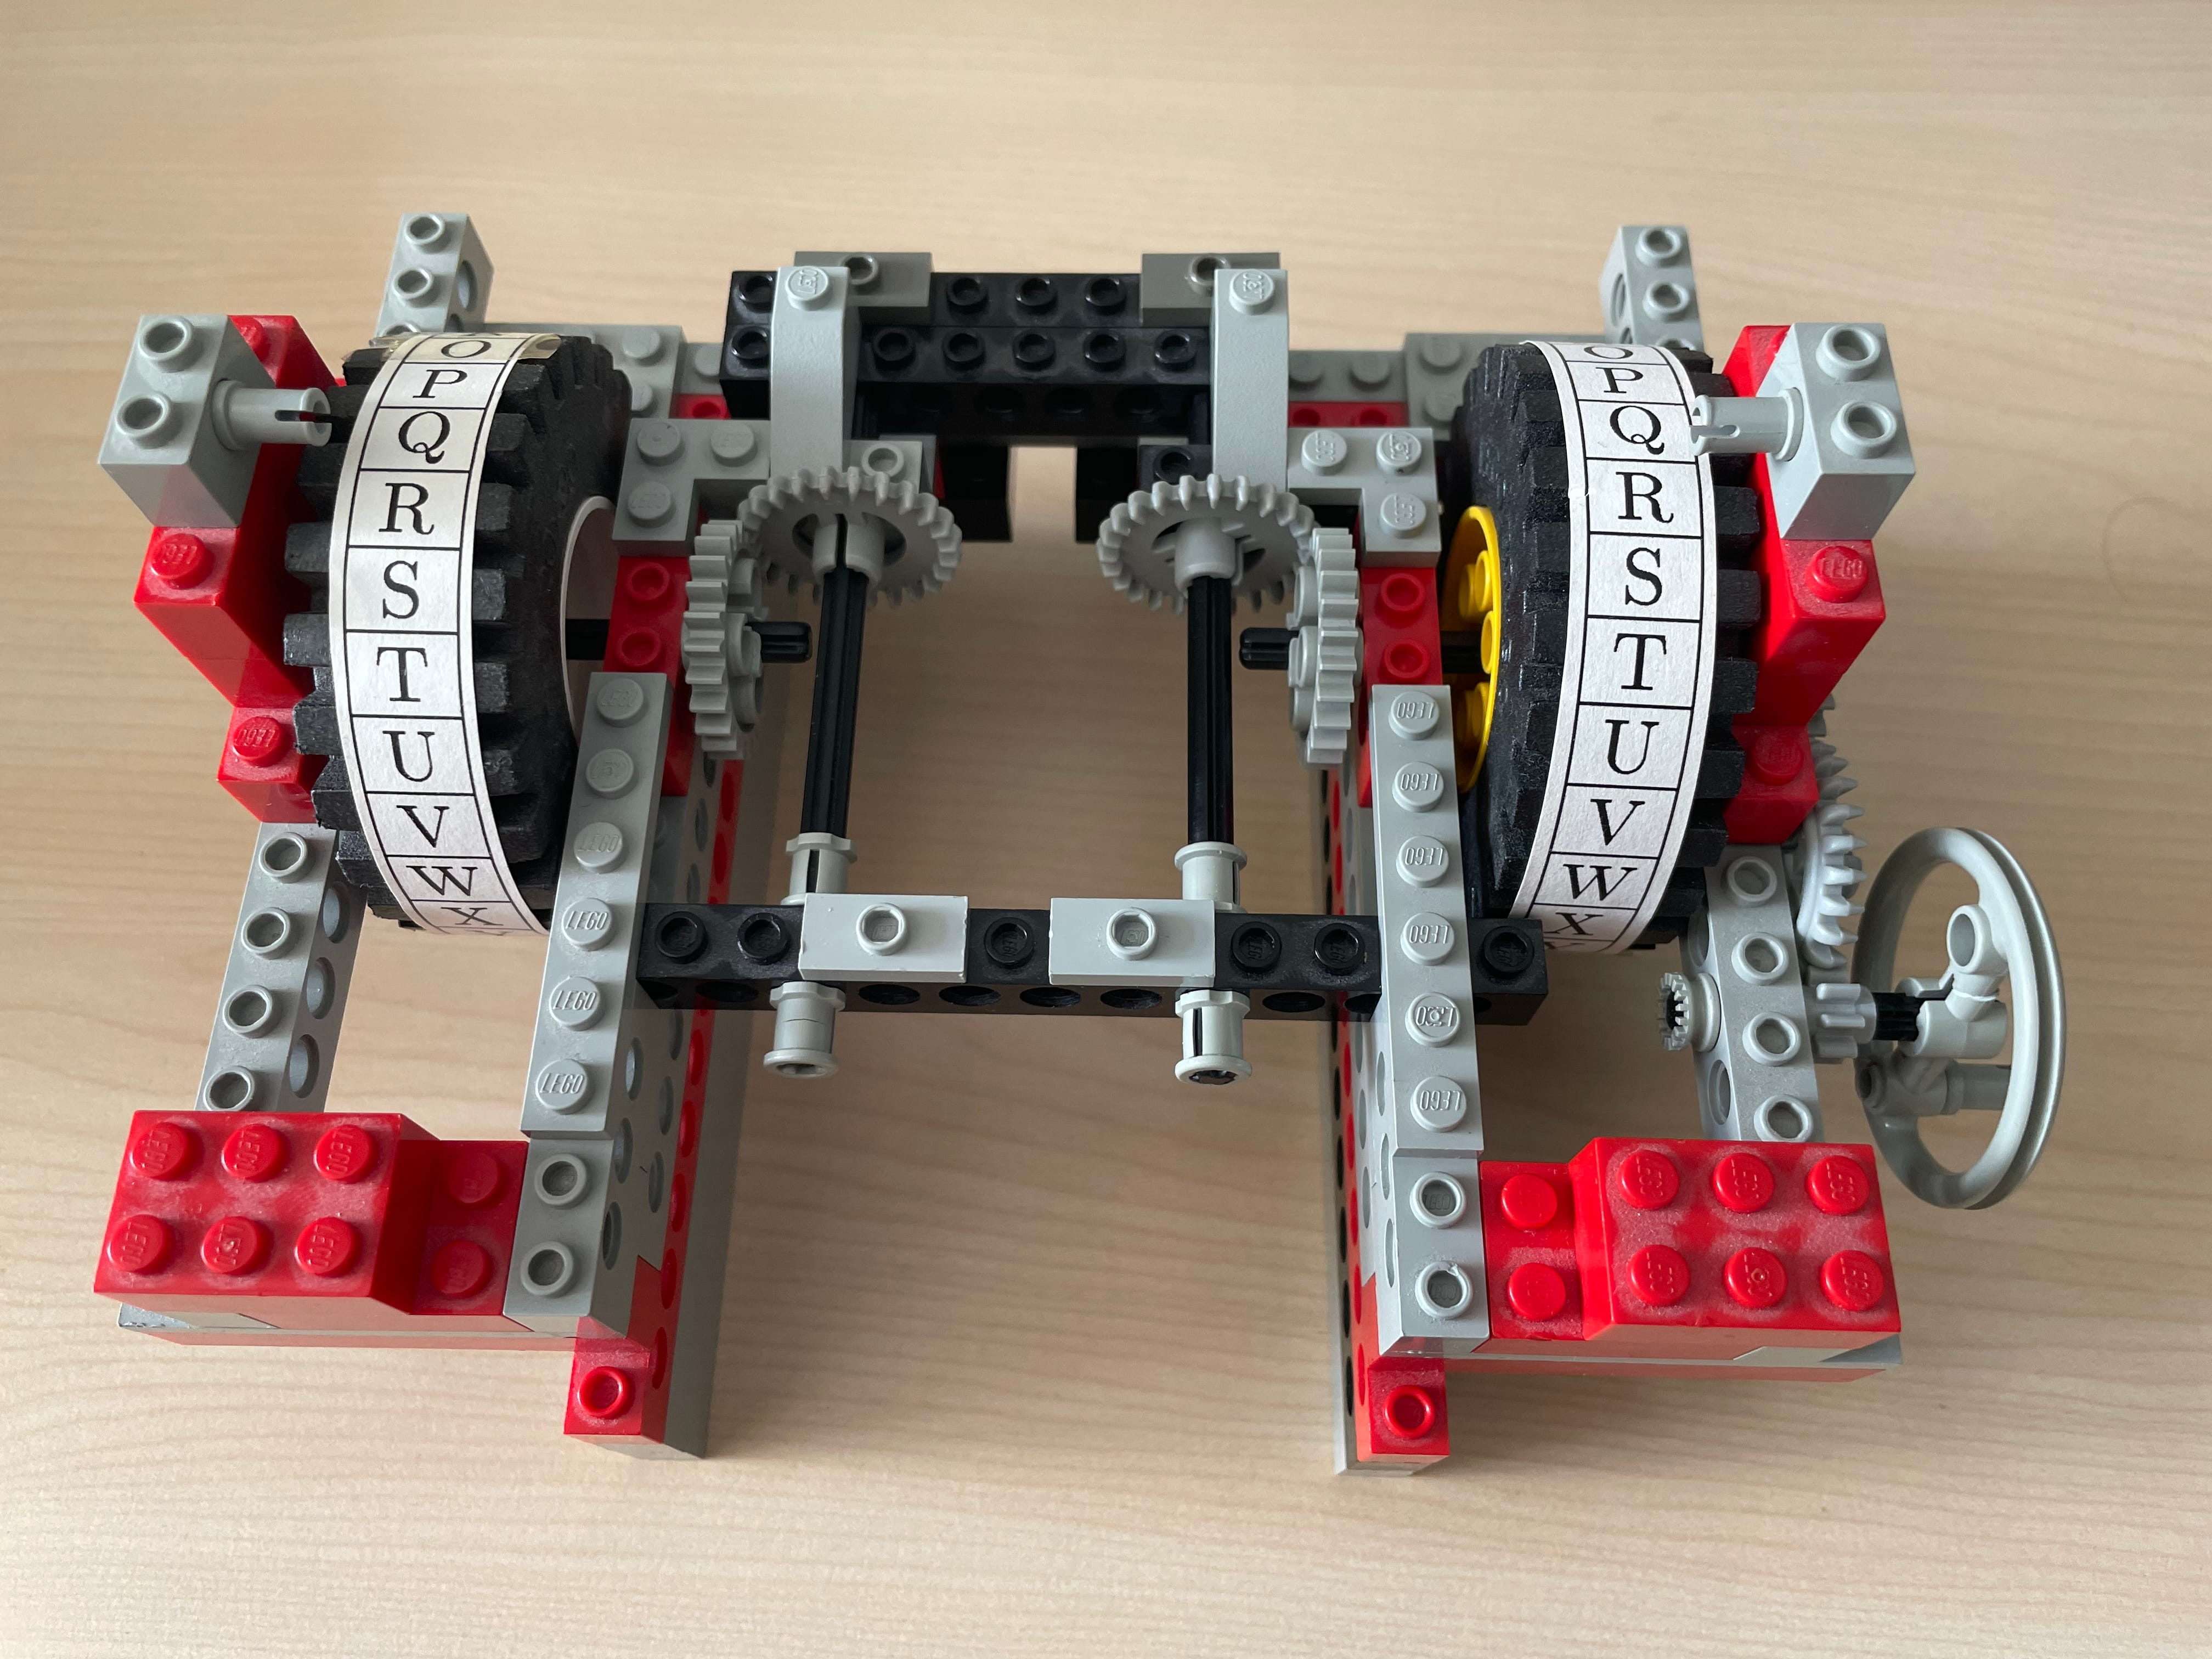
\includegraphics[width=200pt]{./Bilder/Gestell_o.jpg}}
	\end{minipage}
	\begin{minipage}{.5\textwidth}
		\centering
		\psframebox[blur=true,shadow=true]{
			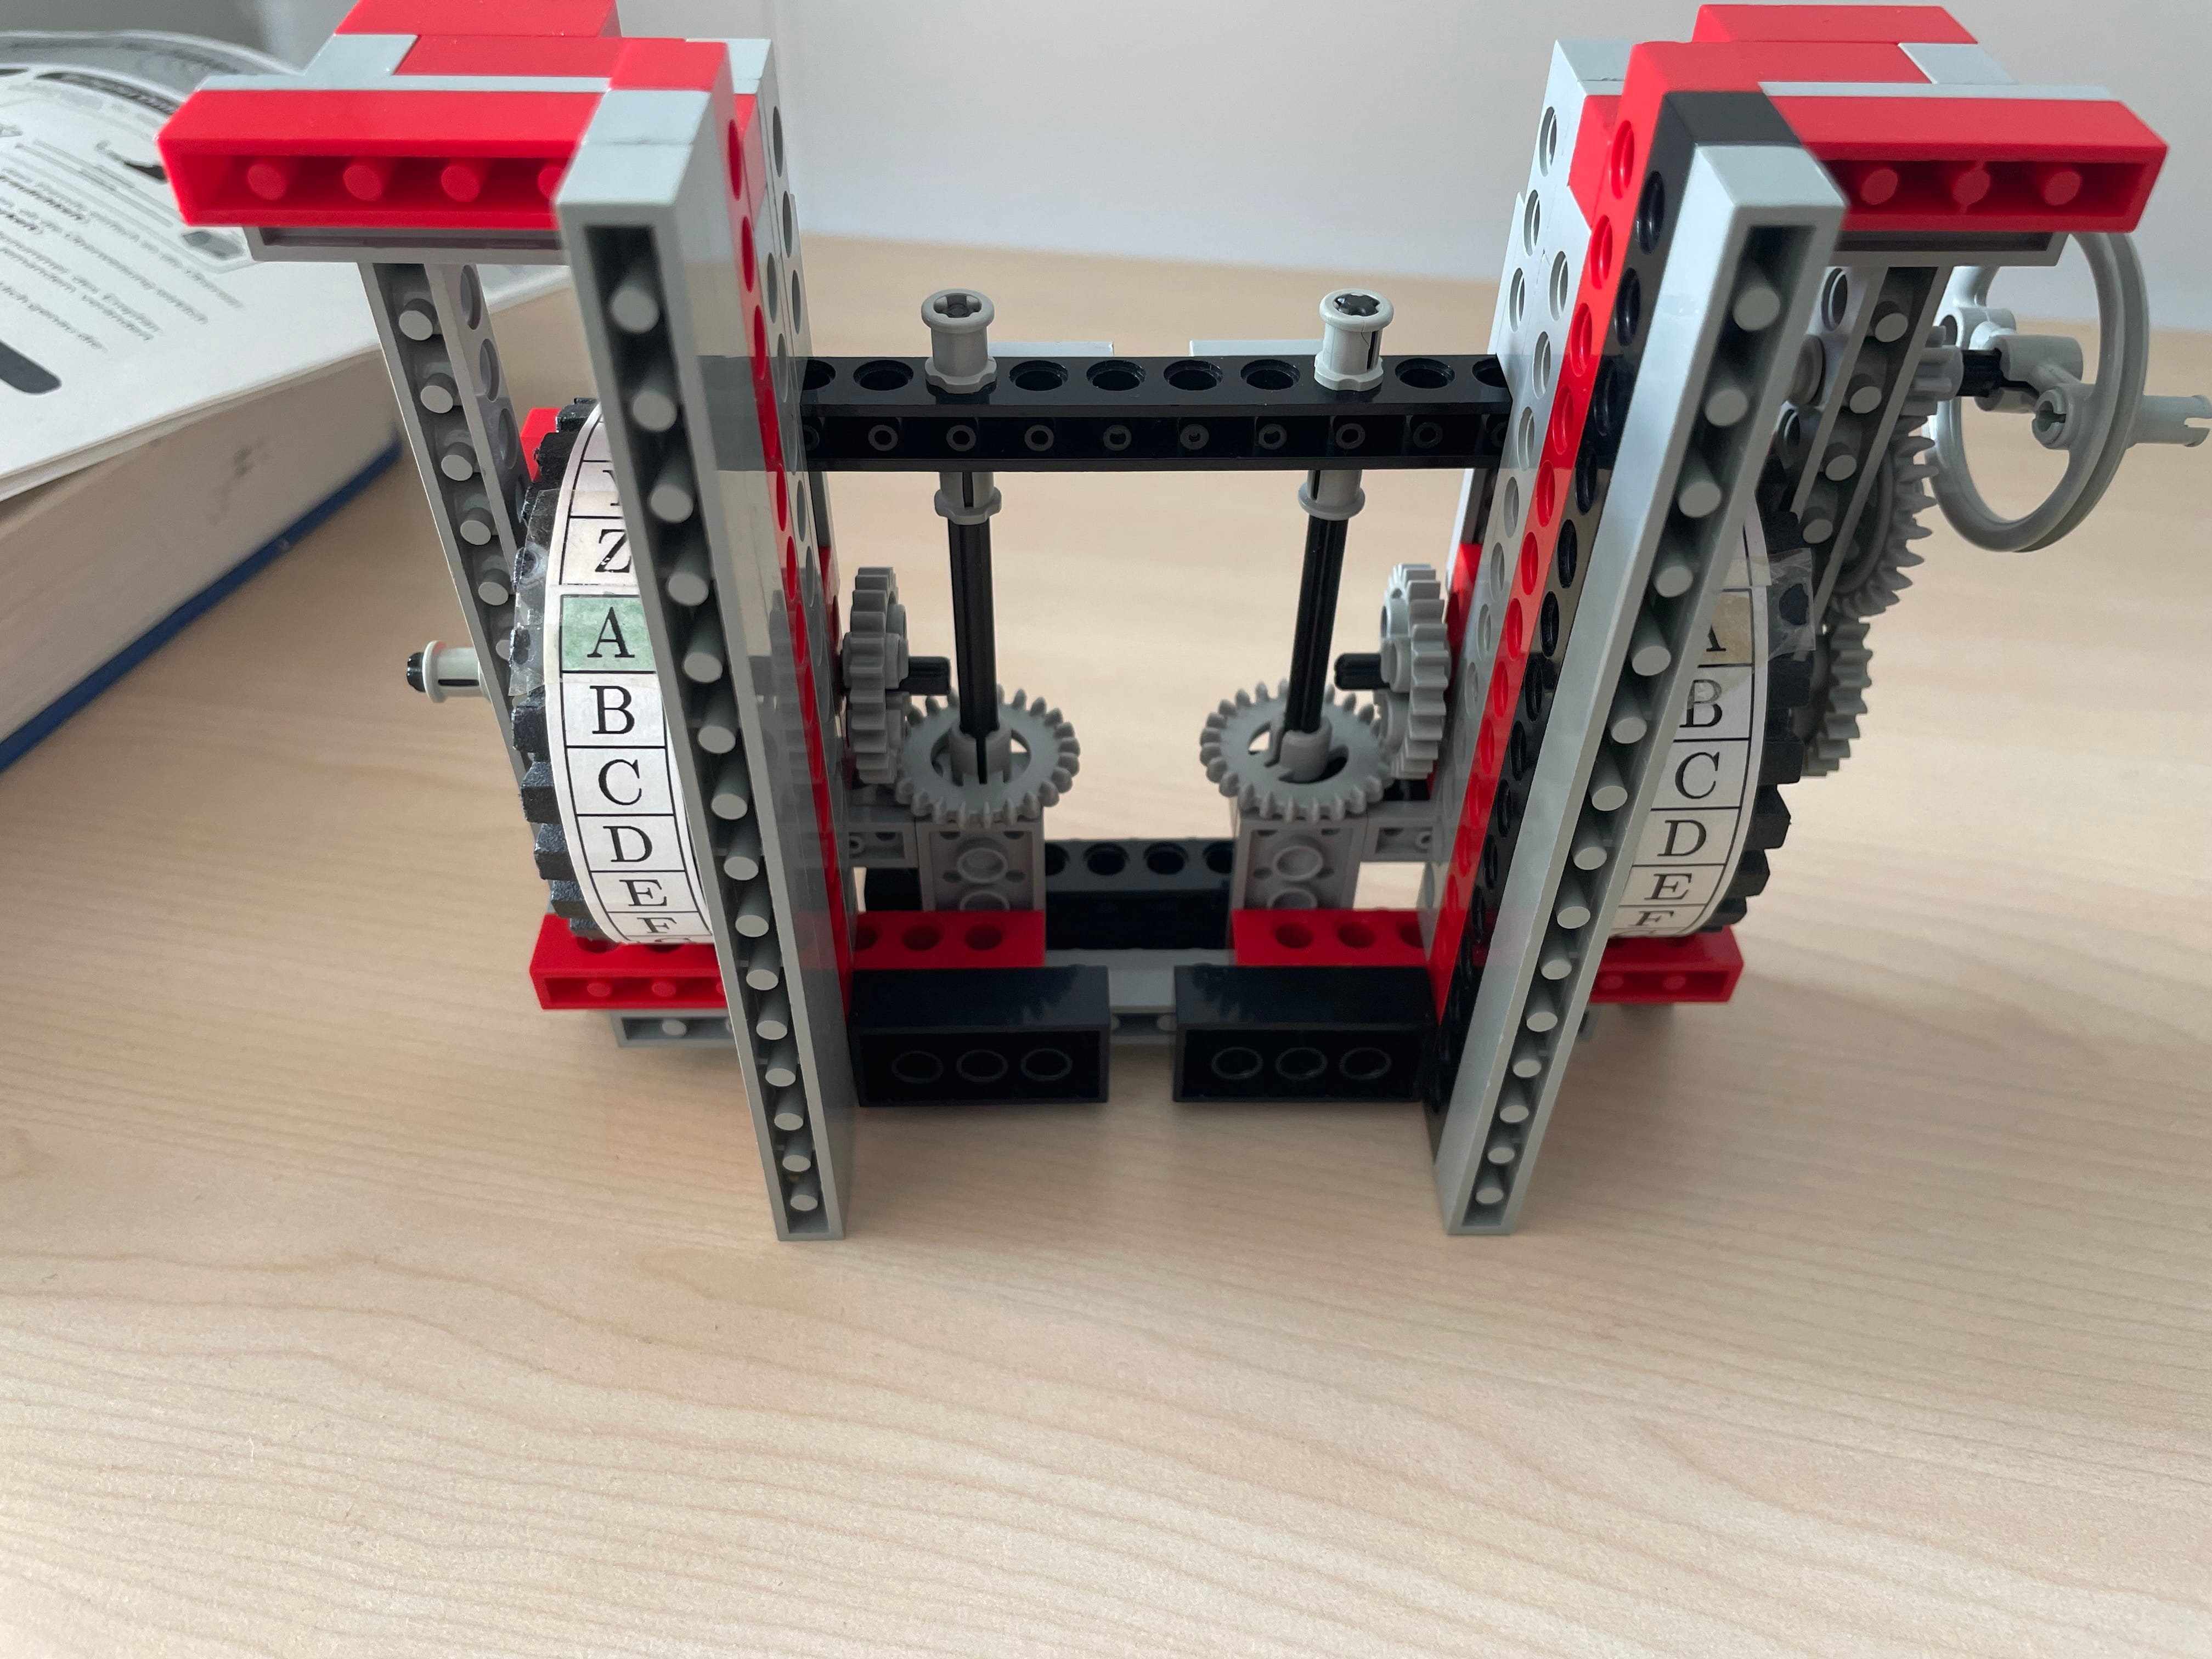
\includegraphics[width=200pt]{./Bilder/Gestell_u.jpg}}
	\end{minipage}
	
	\begin{minipage}{.5\textwidth}
		\centering
		\psframebox[blur=true,shadow=true]{
			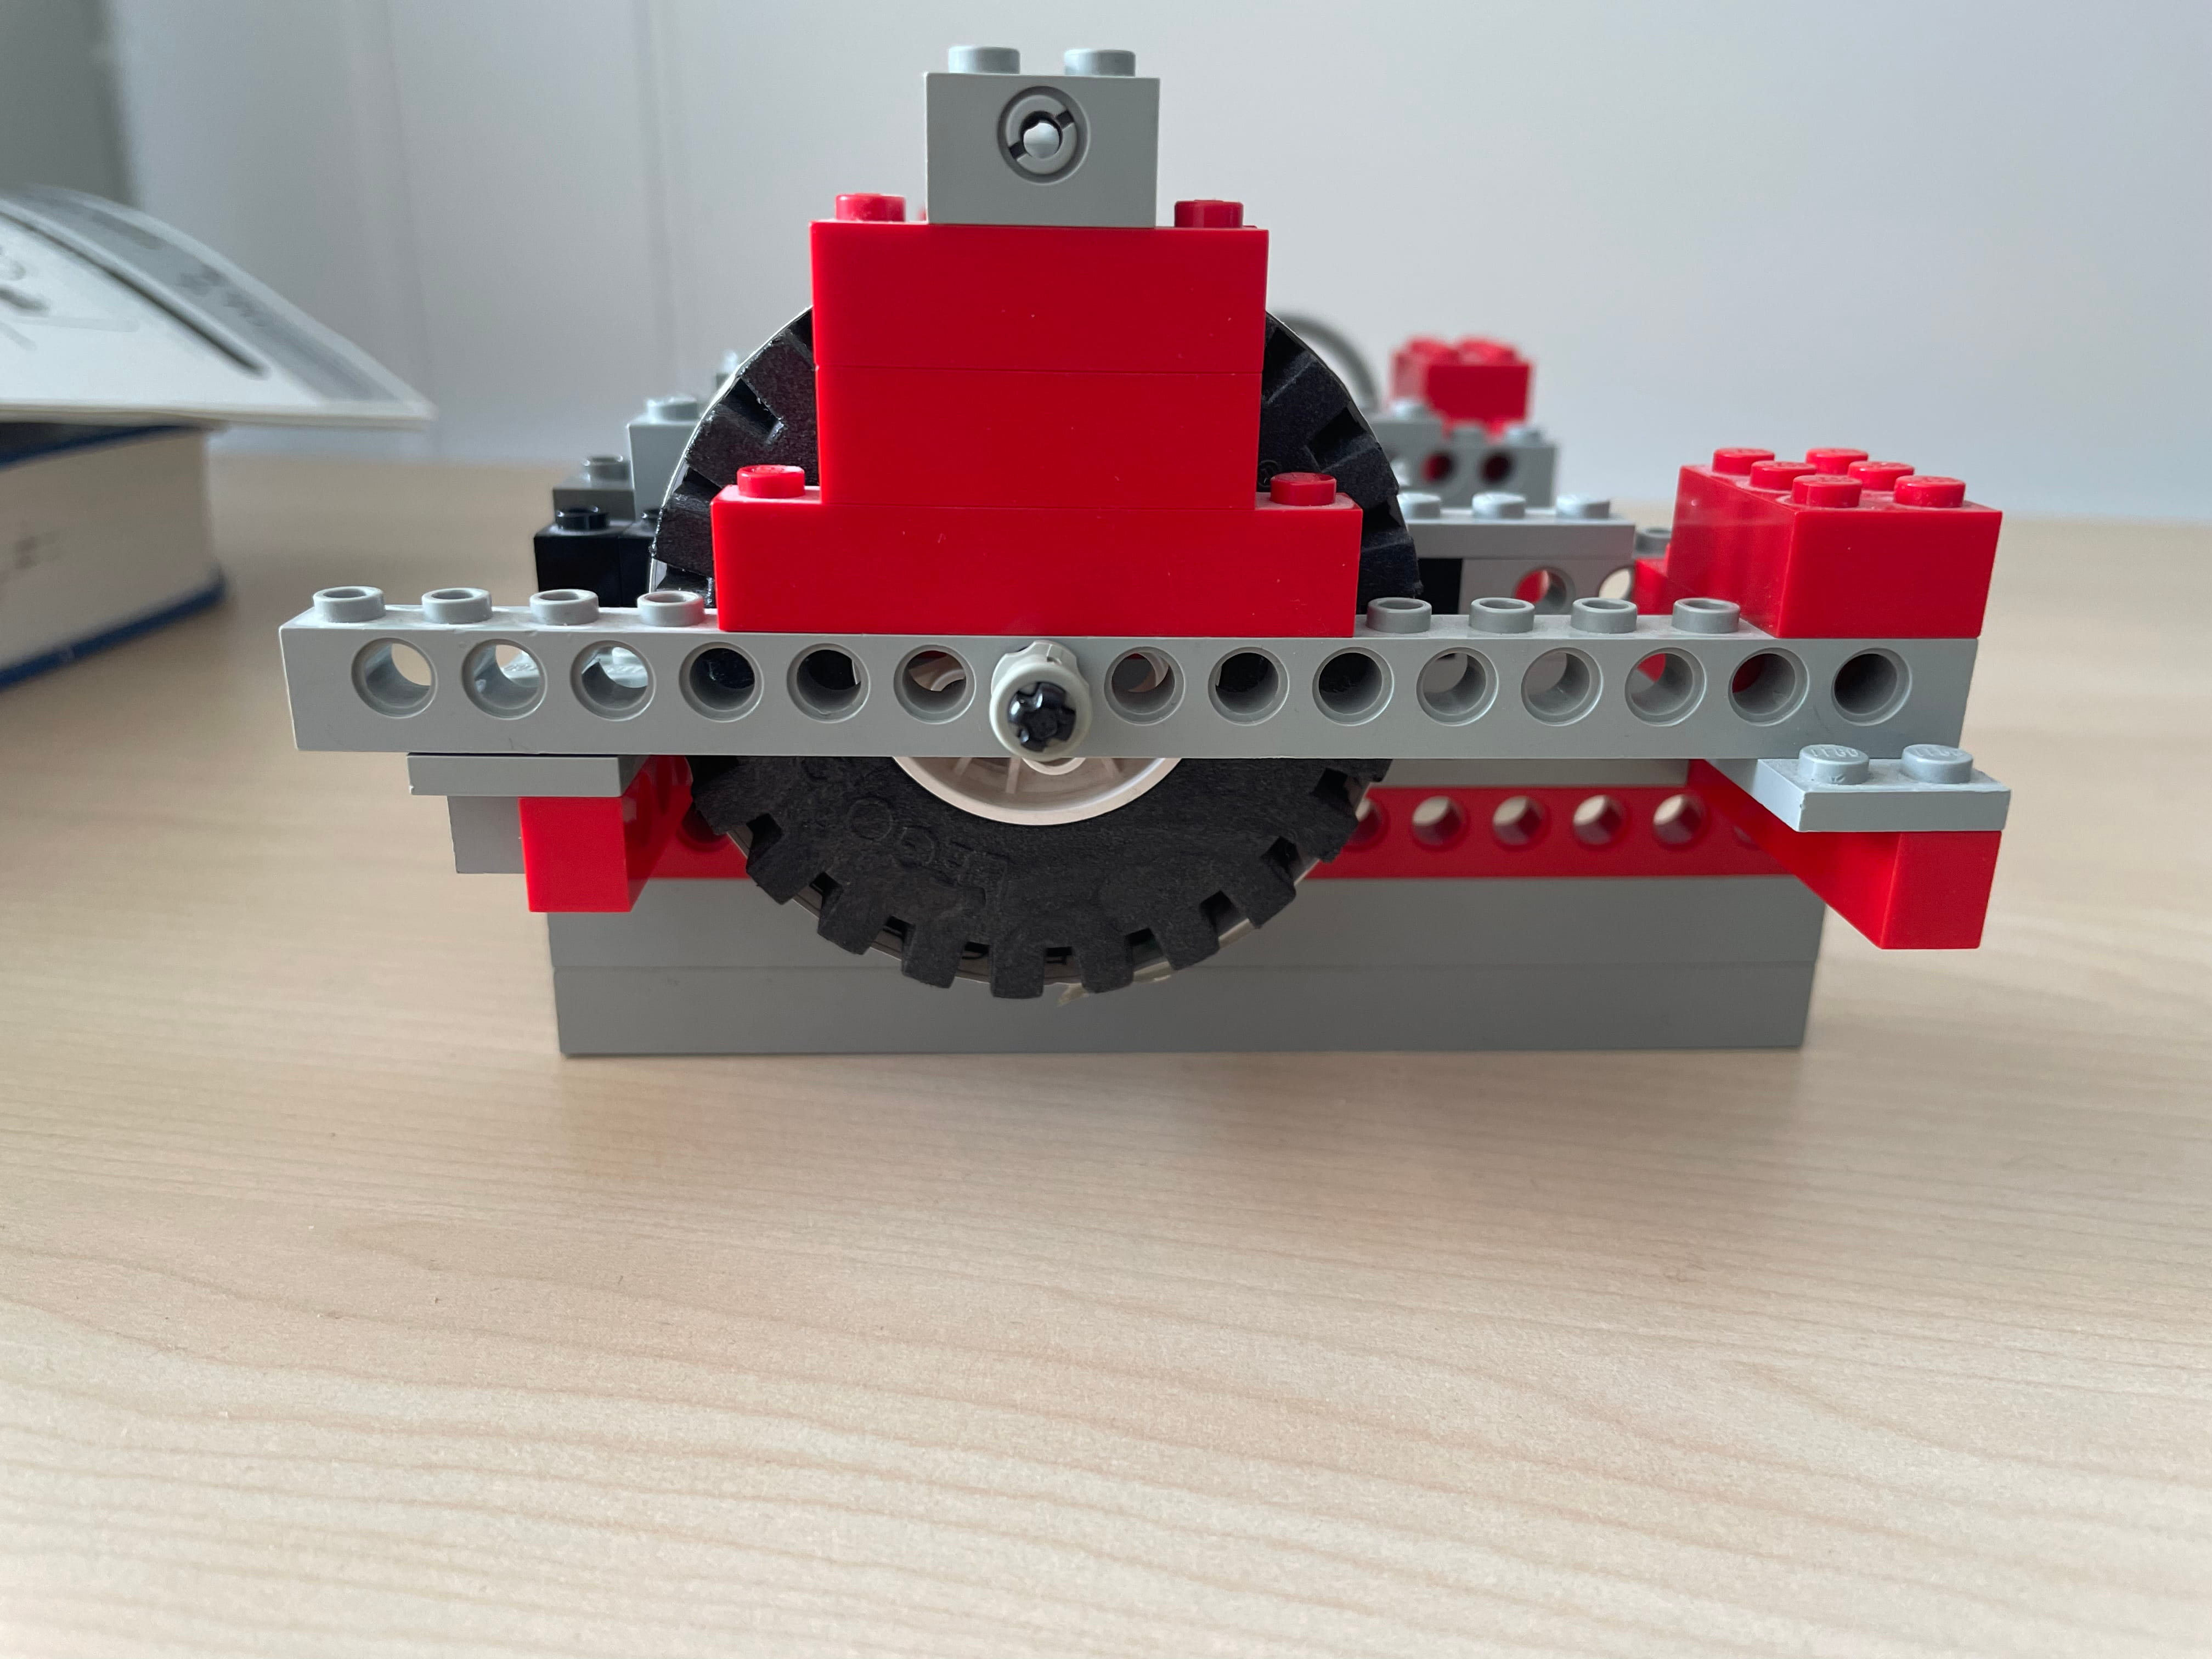
\includegraphics[width=200pt]{./Bilder/Gestell_l.jpg}}
	\end{minipage}
	\begin{minipage}{.5\textwidth}
		\centering
		\psframebox[blur=true,shadow=true]{
			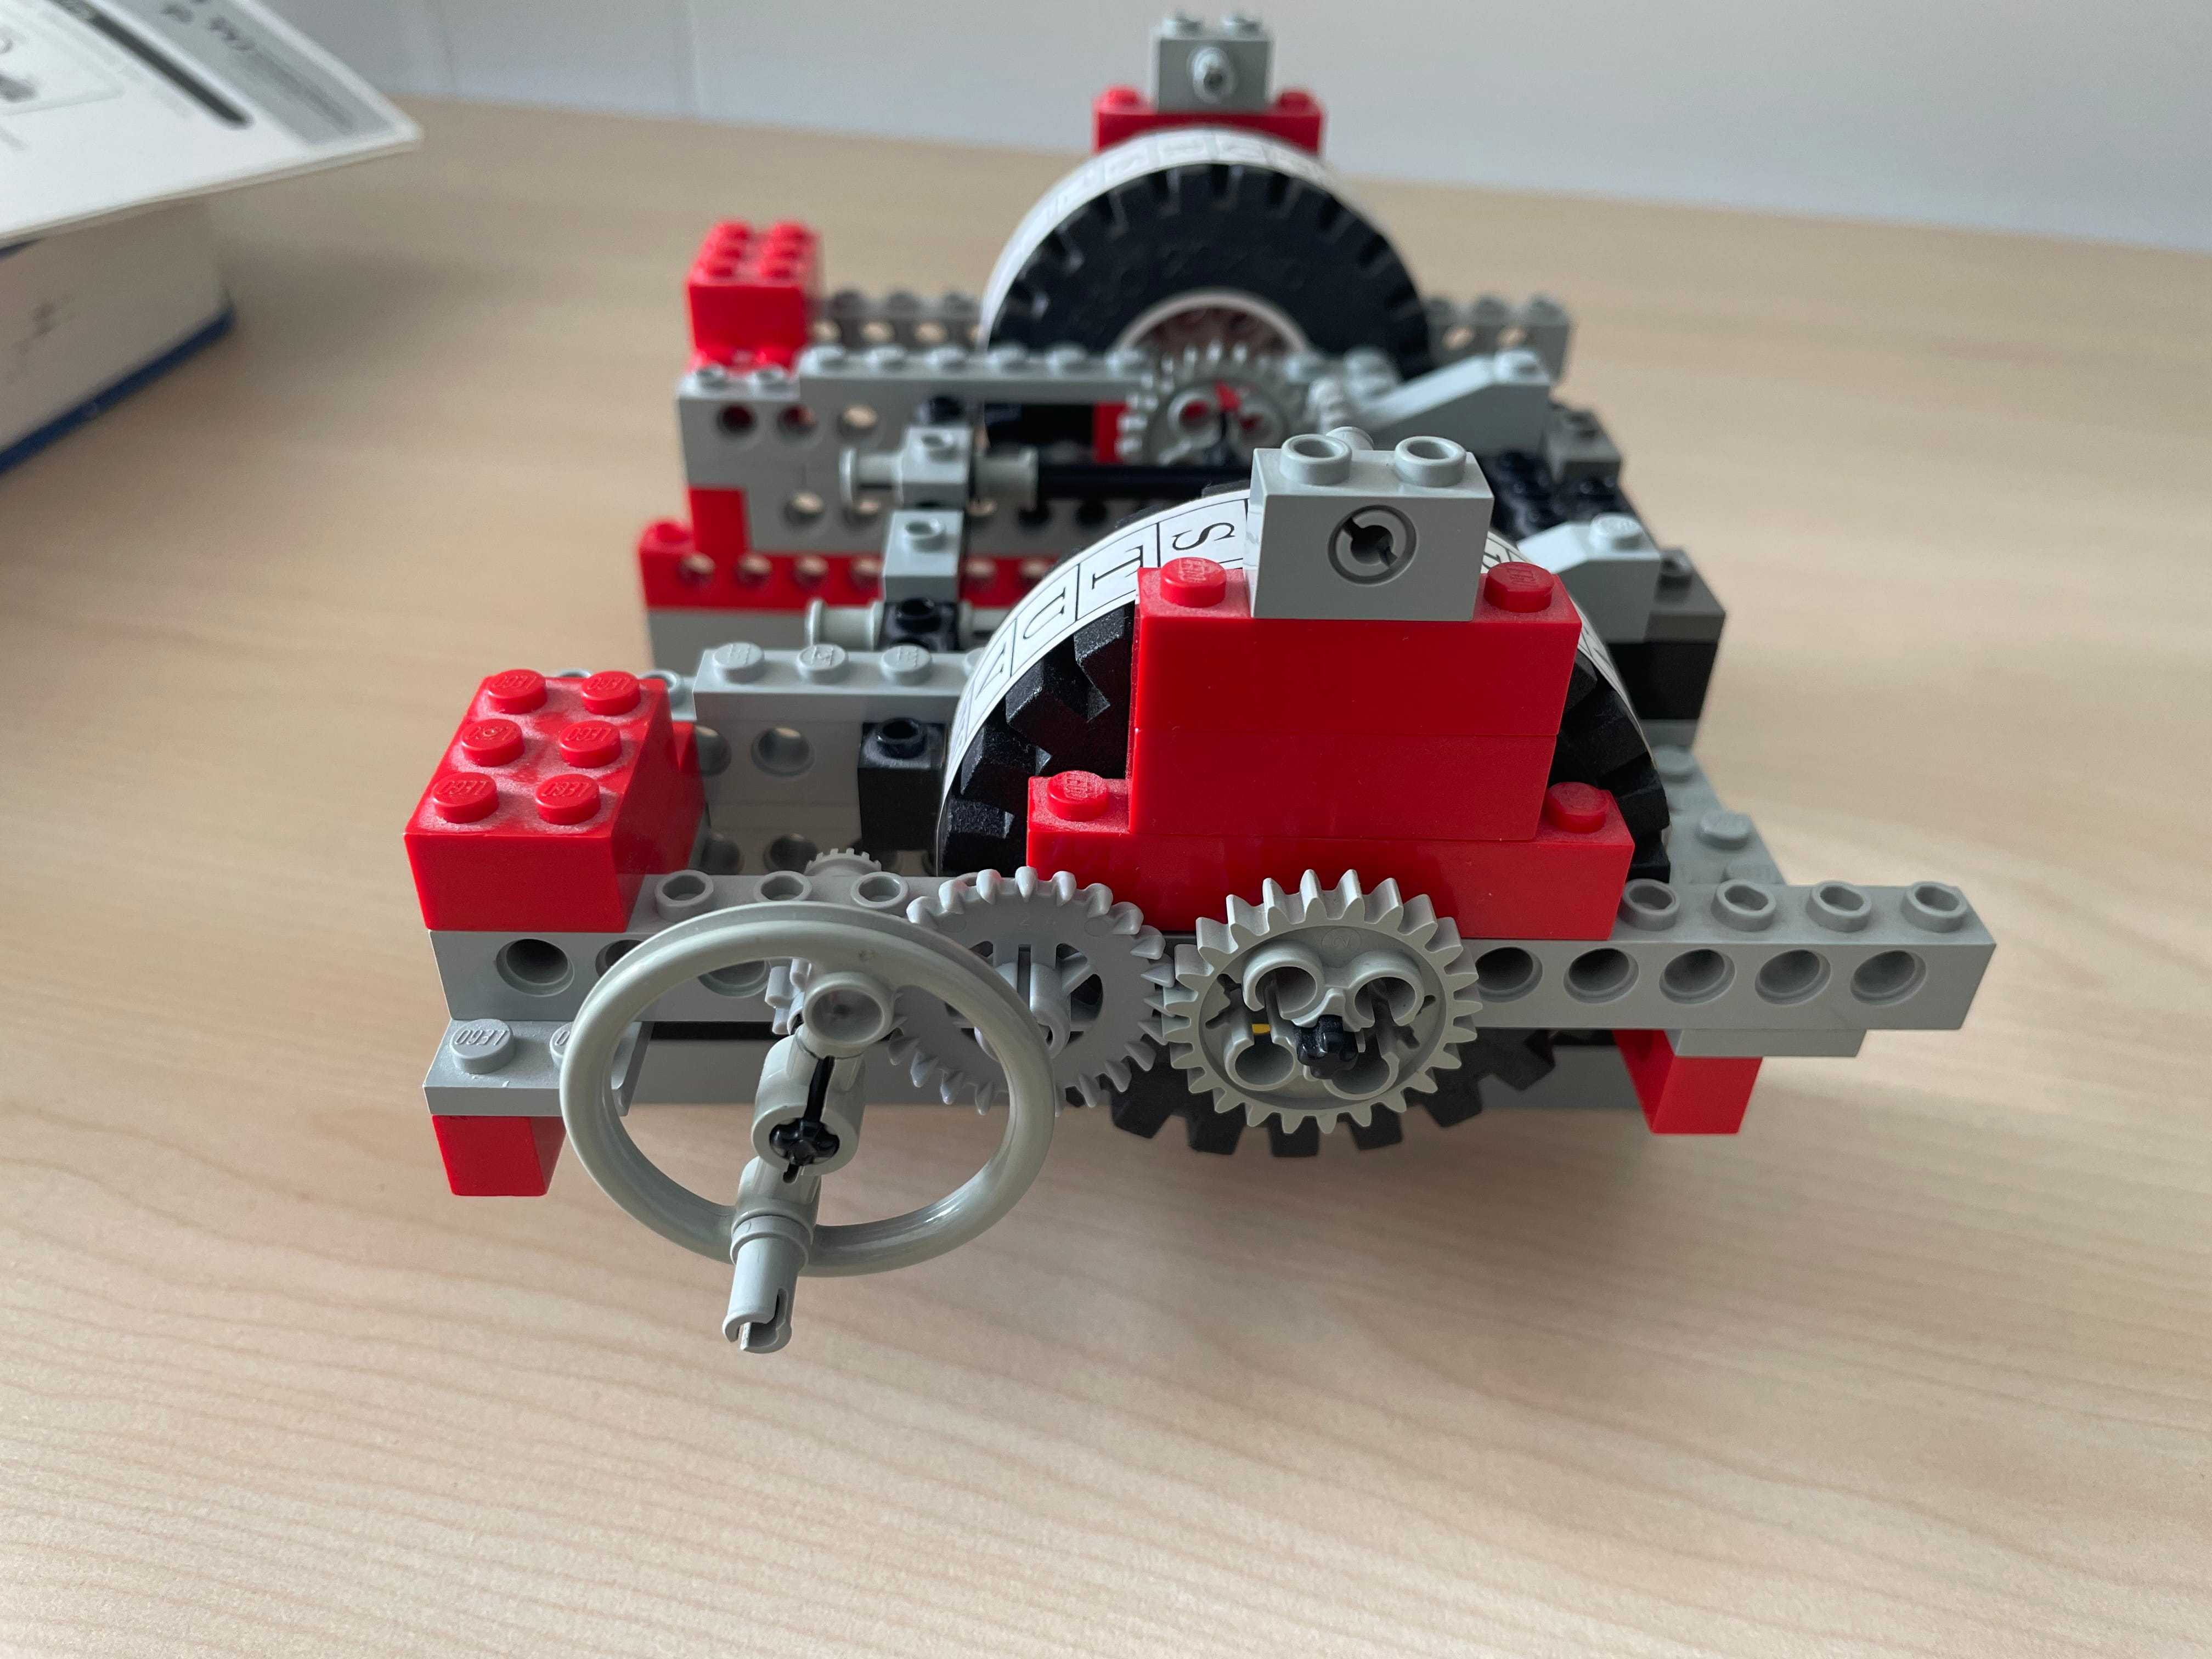
\includegraphics[width=200pt]{./Bilder/Gestell_r.jpg}}
	\end{minipage}
	
	\begin{minipage}{.5\textwidth}
		\centering
		\psframebox[blur=true,shadow=true]{
			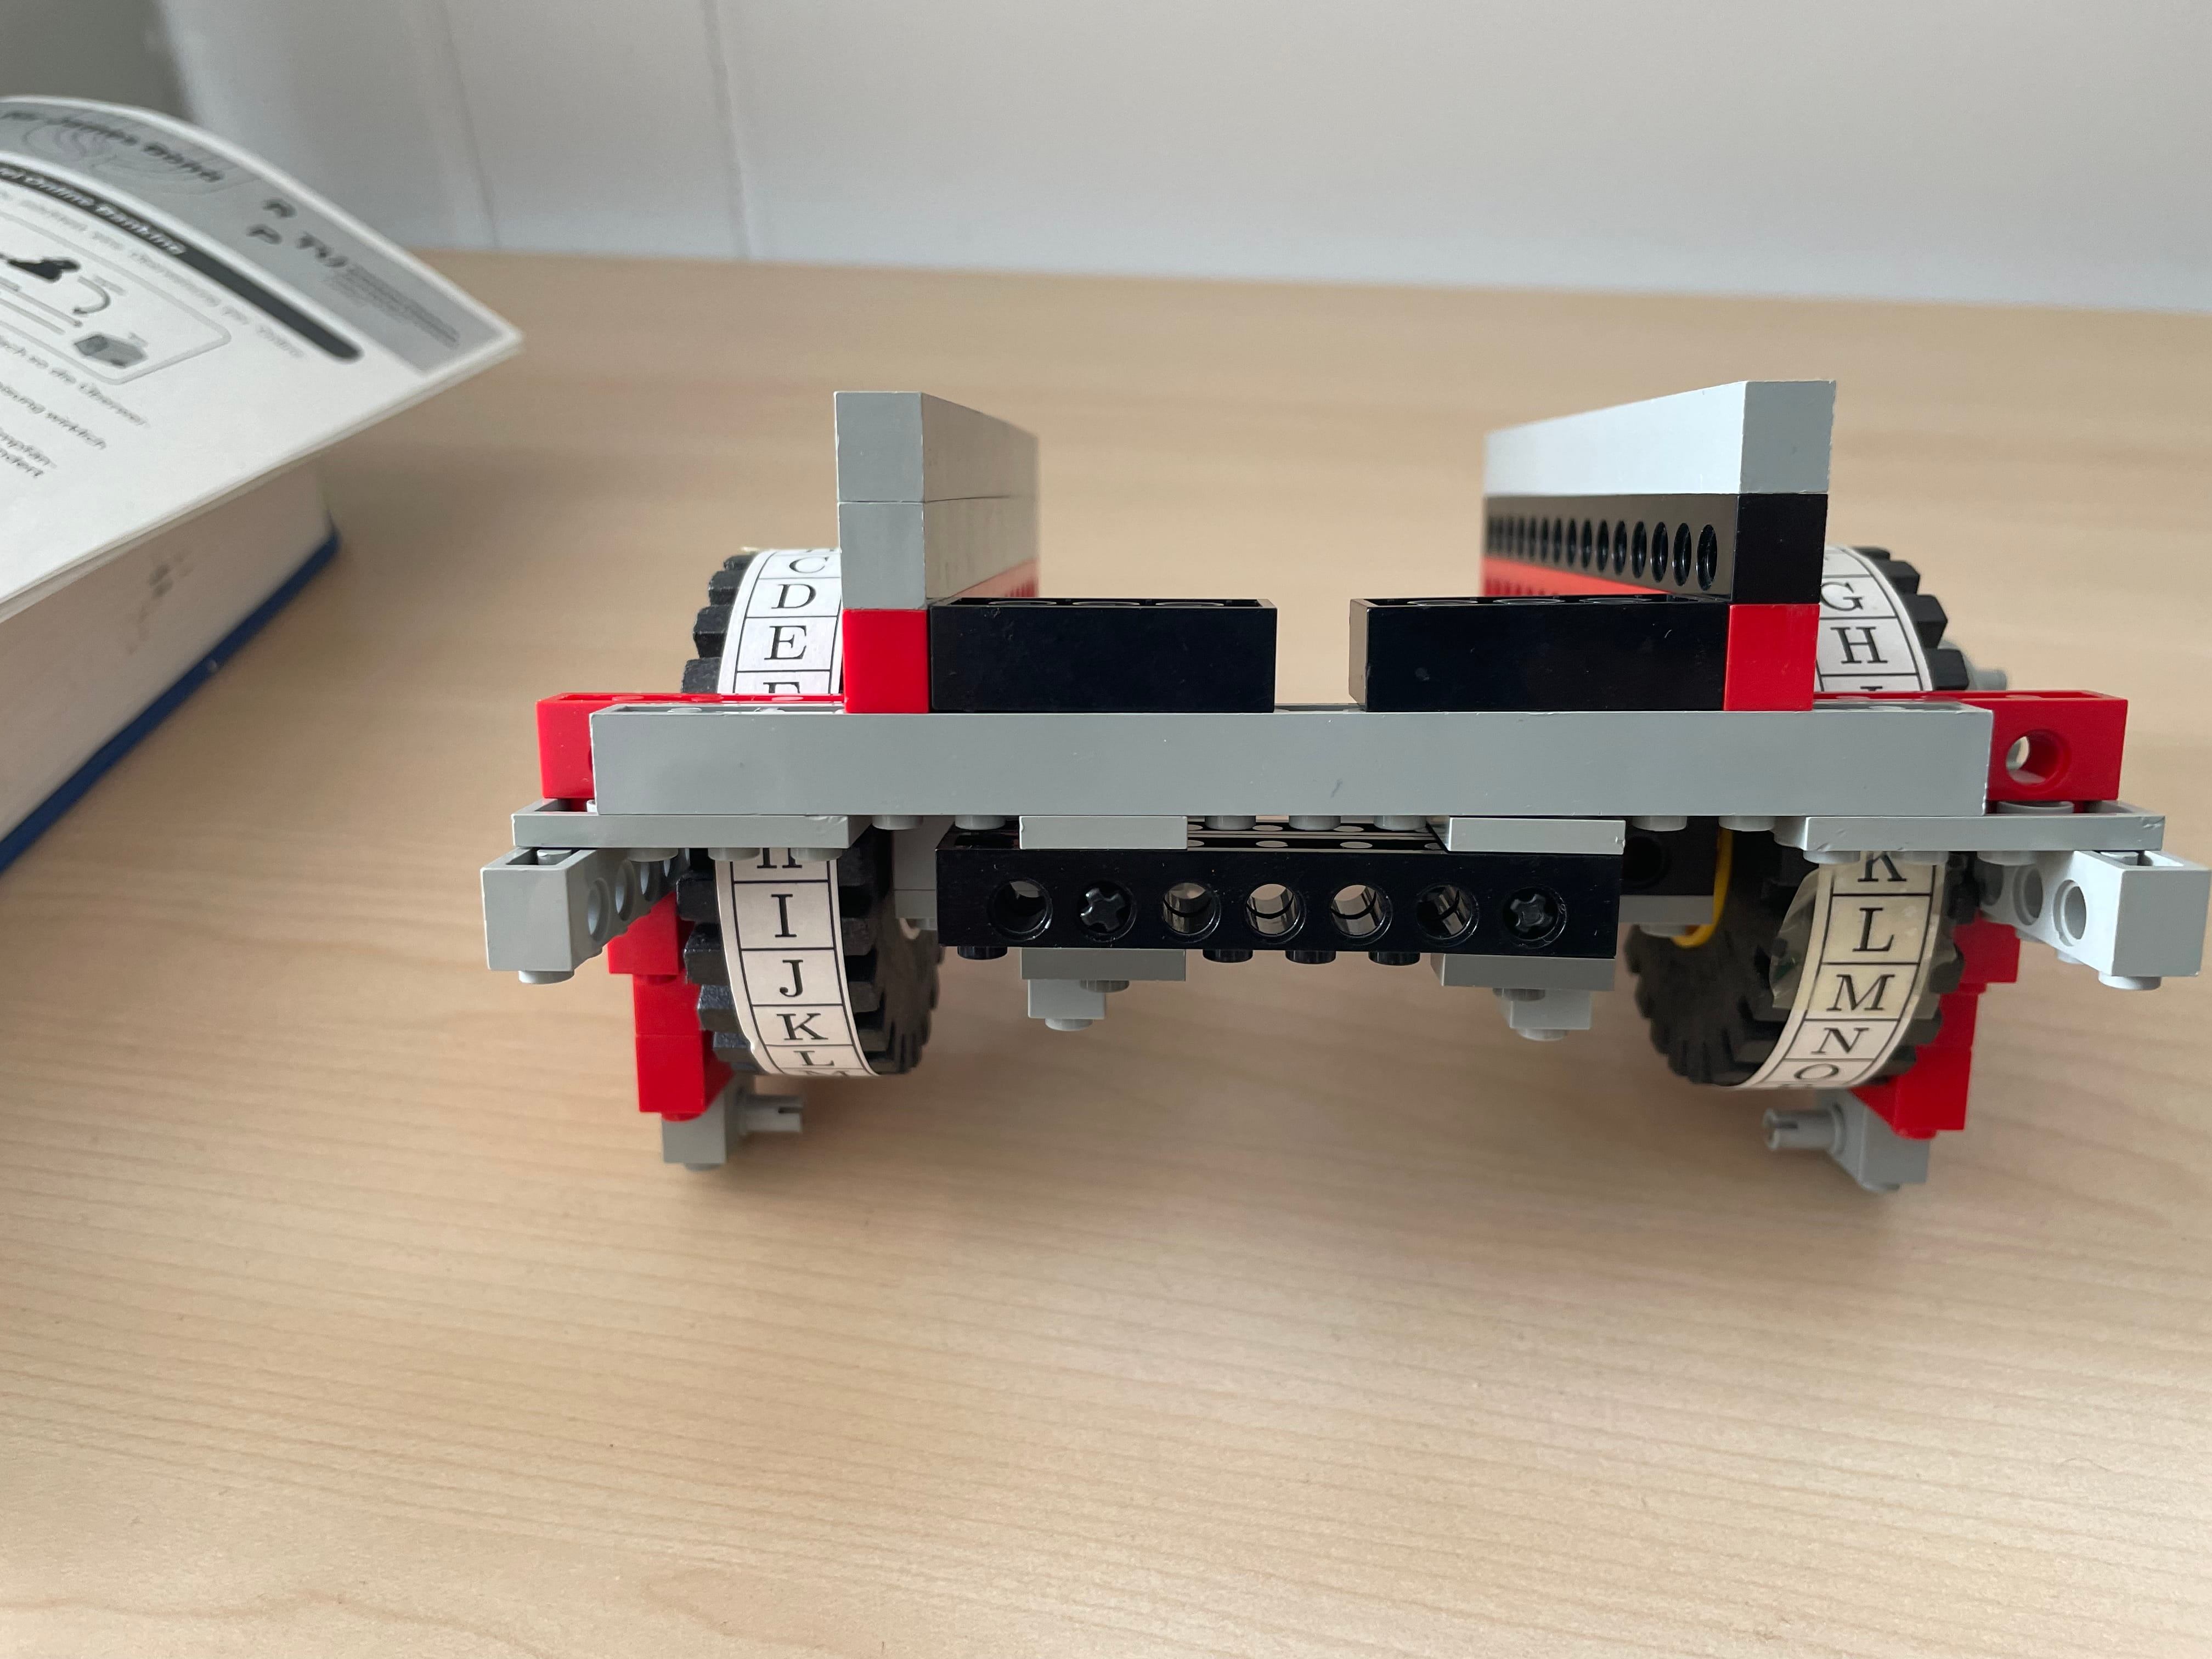
\includegraphics[width=200pt]{./Bilder/Gestell_h.jpg}}
	\end{minipage}
	\begin{minipage}{.5\textwidth}
		\centering
		\psframebox[blur=true,shadow=true]{
			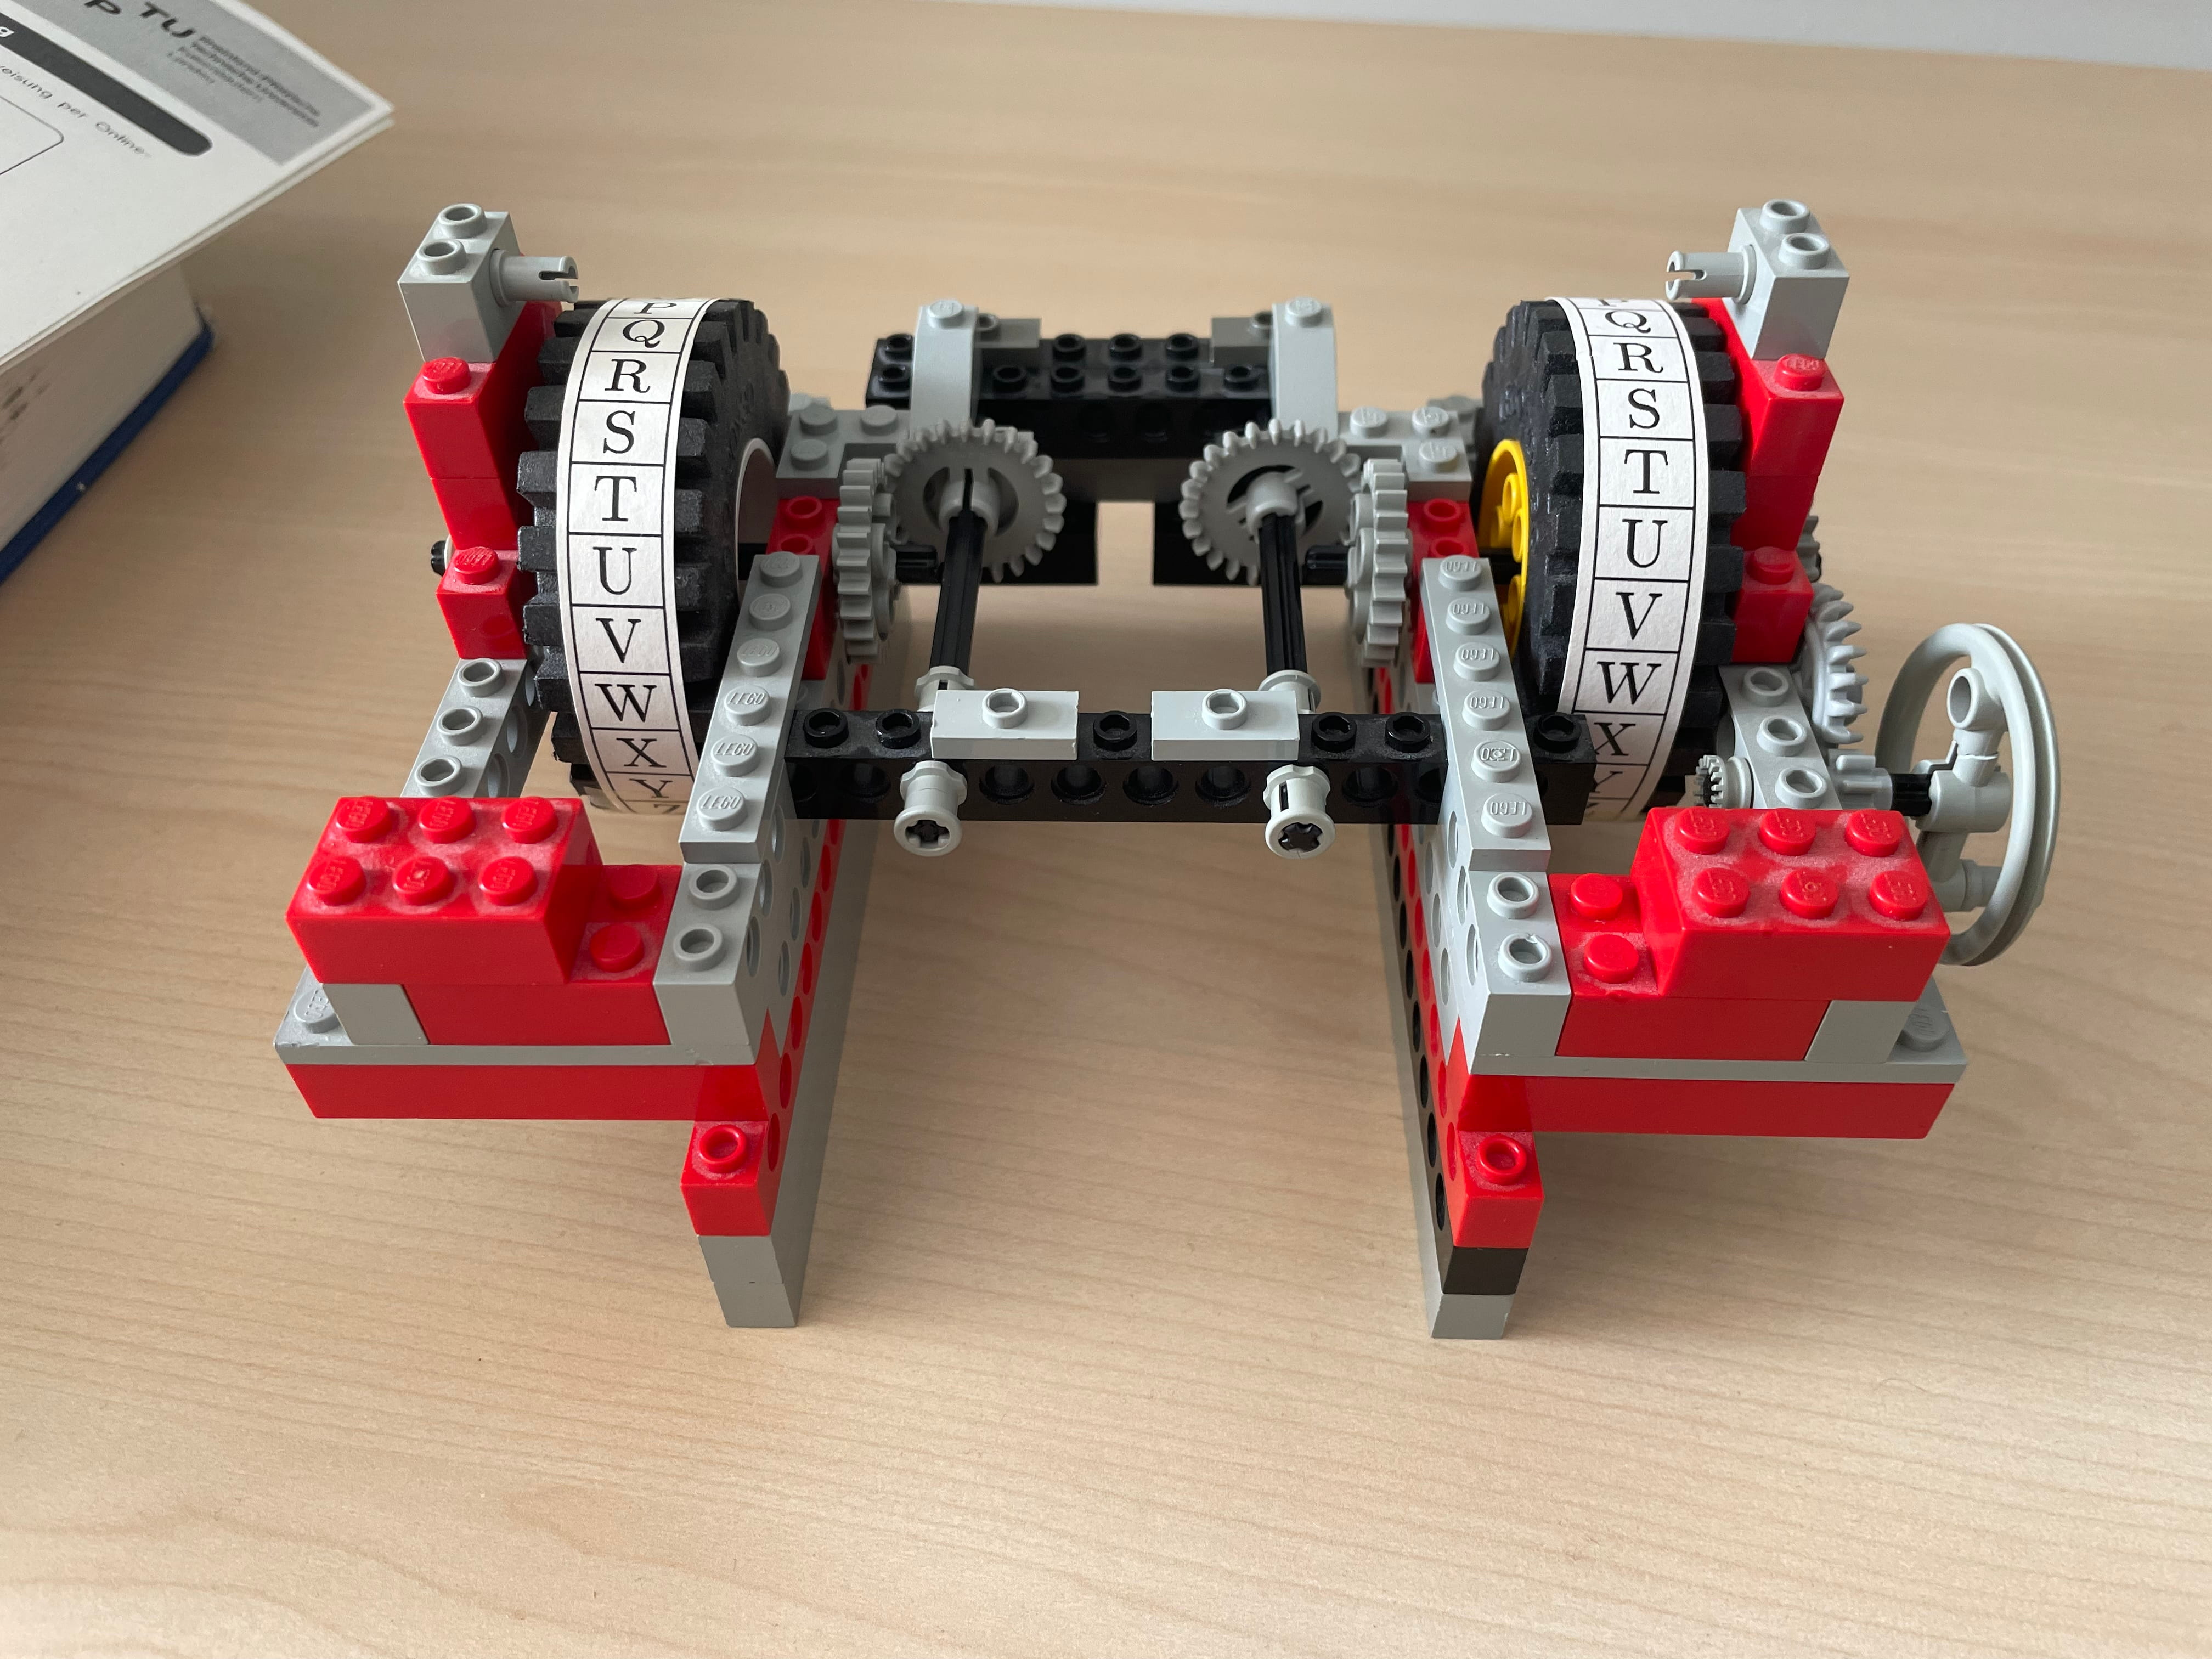
\includegraphics[width=200pt]{./Bilder/Gestell_v.jpg}}
	\end{minipage}
	
	\vspace{1em}
	Das Zusammensetzten erfolgt nach der separaten Konstruktion aller drei Teile.
	\begin{enumerate}[font=\sffamily\bfseries,leftmargin=*,itemsep=.4\baselineskip,label=\framebox{\arabic*.}]
		\item Den Hebel entsprechend wie auf Fig. 1 auf die grüne Platine setzten.
		\item Das Gestell mit zwei Noppen Abstand vom Hebel auf die grüne Platine setzten (Fig. 13).
		\item Das Gestell zwischen den Zahnrädern einfädeln und an den Seiten festmachen. Aufpassen, dass der Hebel entsprechend des letzten Bildes eingefädelt wird (Fig. 14).
	\end{enumerate}
	\newpage
	\textsc{Der Zusammenbau}
	
	\begin{figure}[h!]
		\begin{minipage}{.5\textwidth}
		\centering
		\psframebox[blur=true,shadow=true]{
			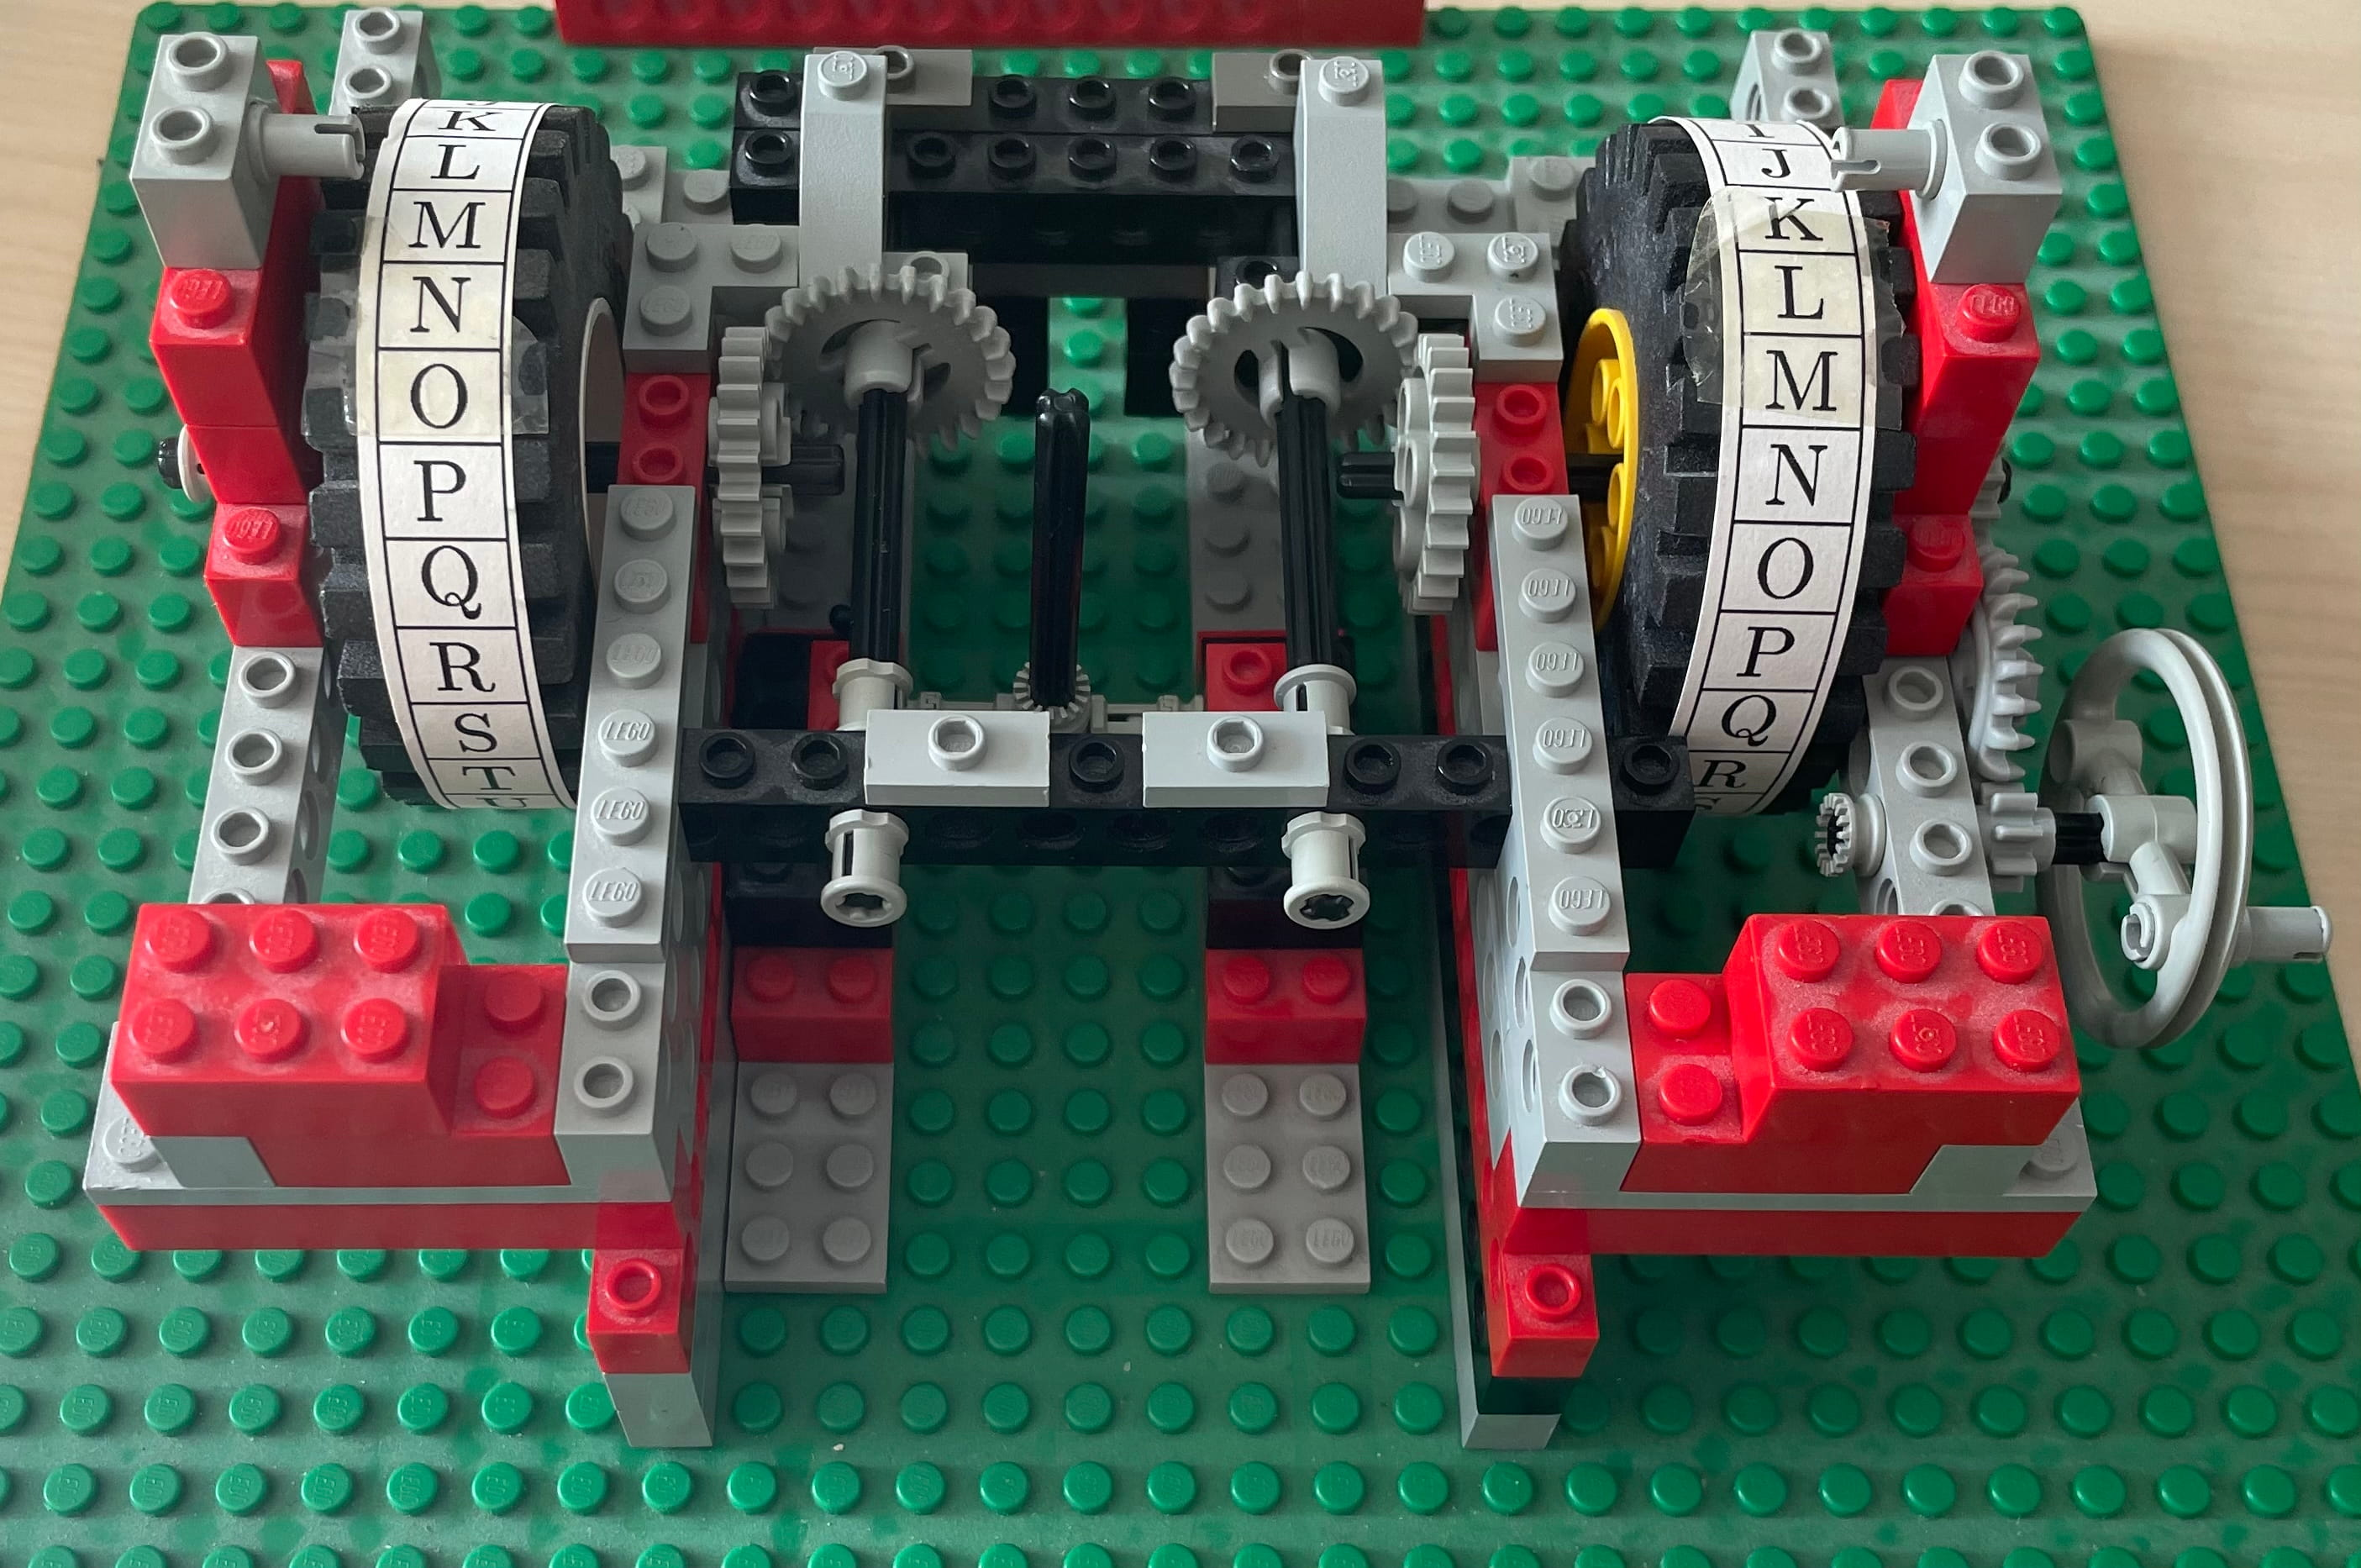
\includegraphics[width=200pt]{./Bilder/Hebel+Gestell_v.jpg}}
		\setcounter{figure}{12}\caption{Hebel mit Gestell.}
	\end{minipage}
	\begin{minipage}{.5\textwidth}
		\centering
		\psframebox[blur=true,shadow=true]{
			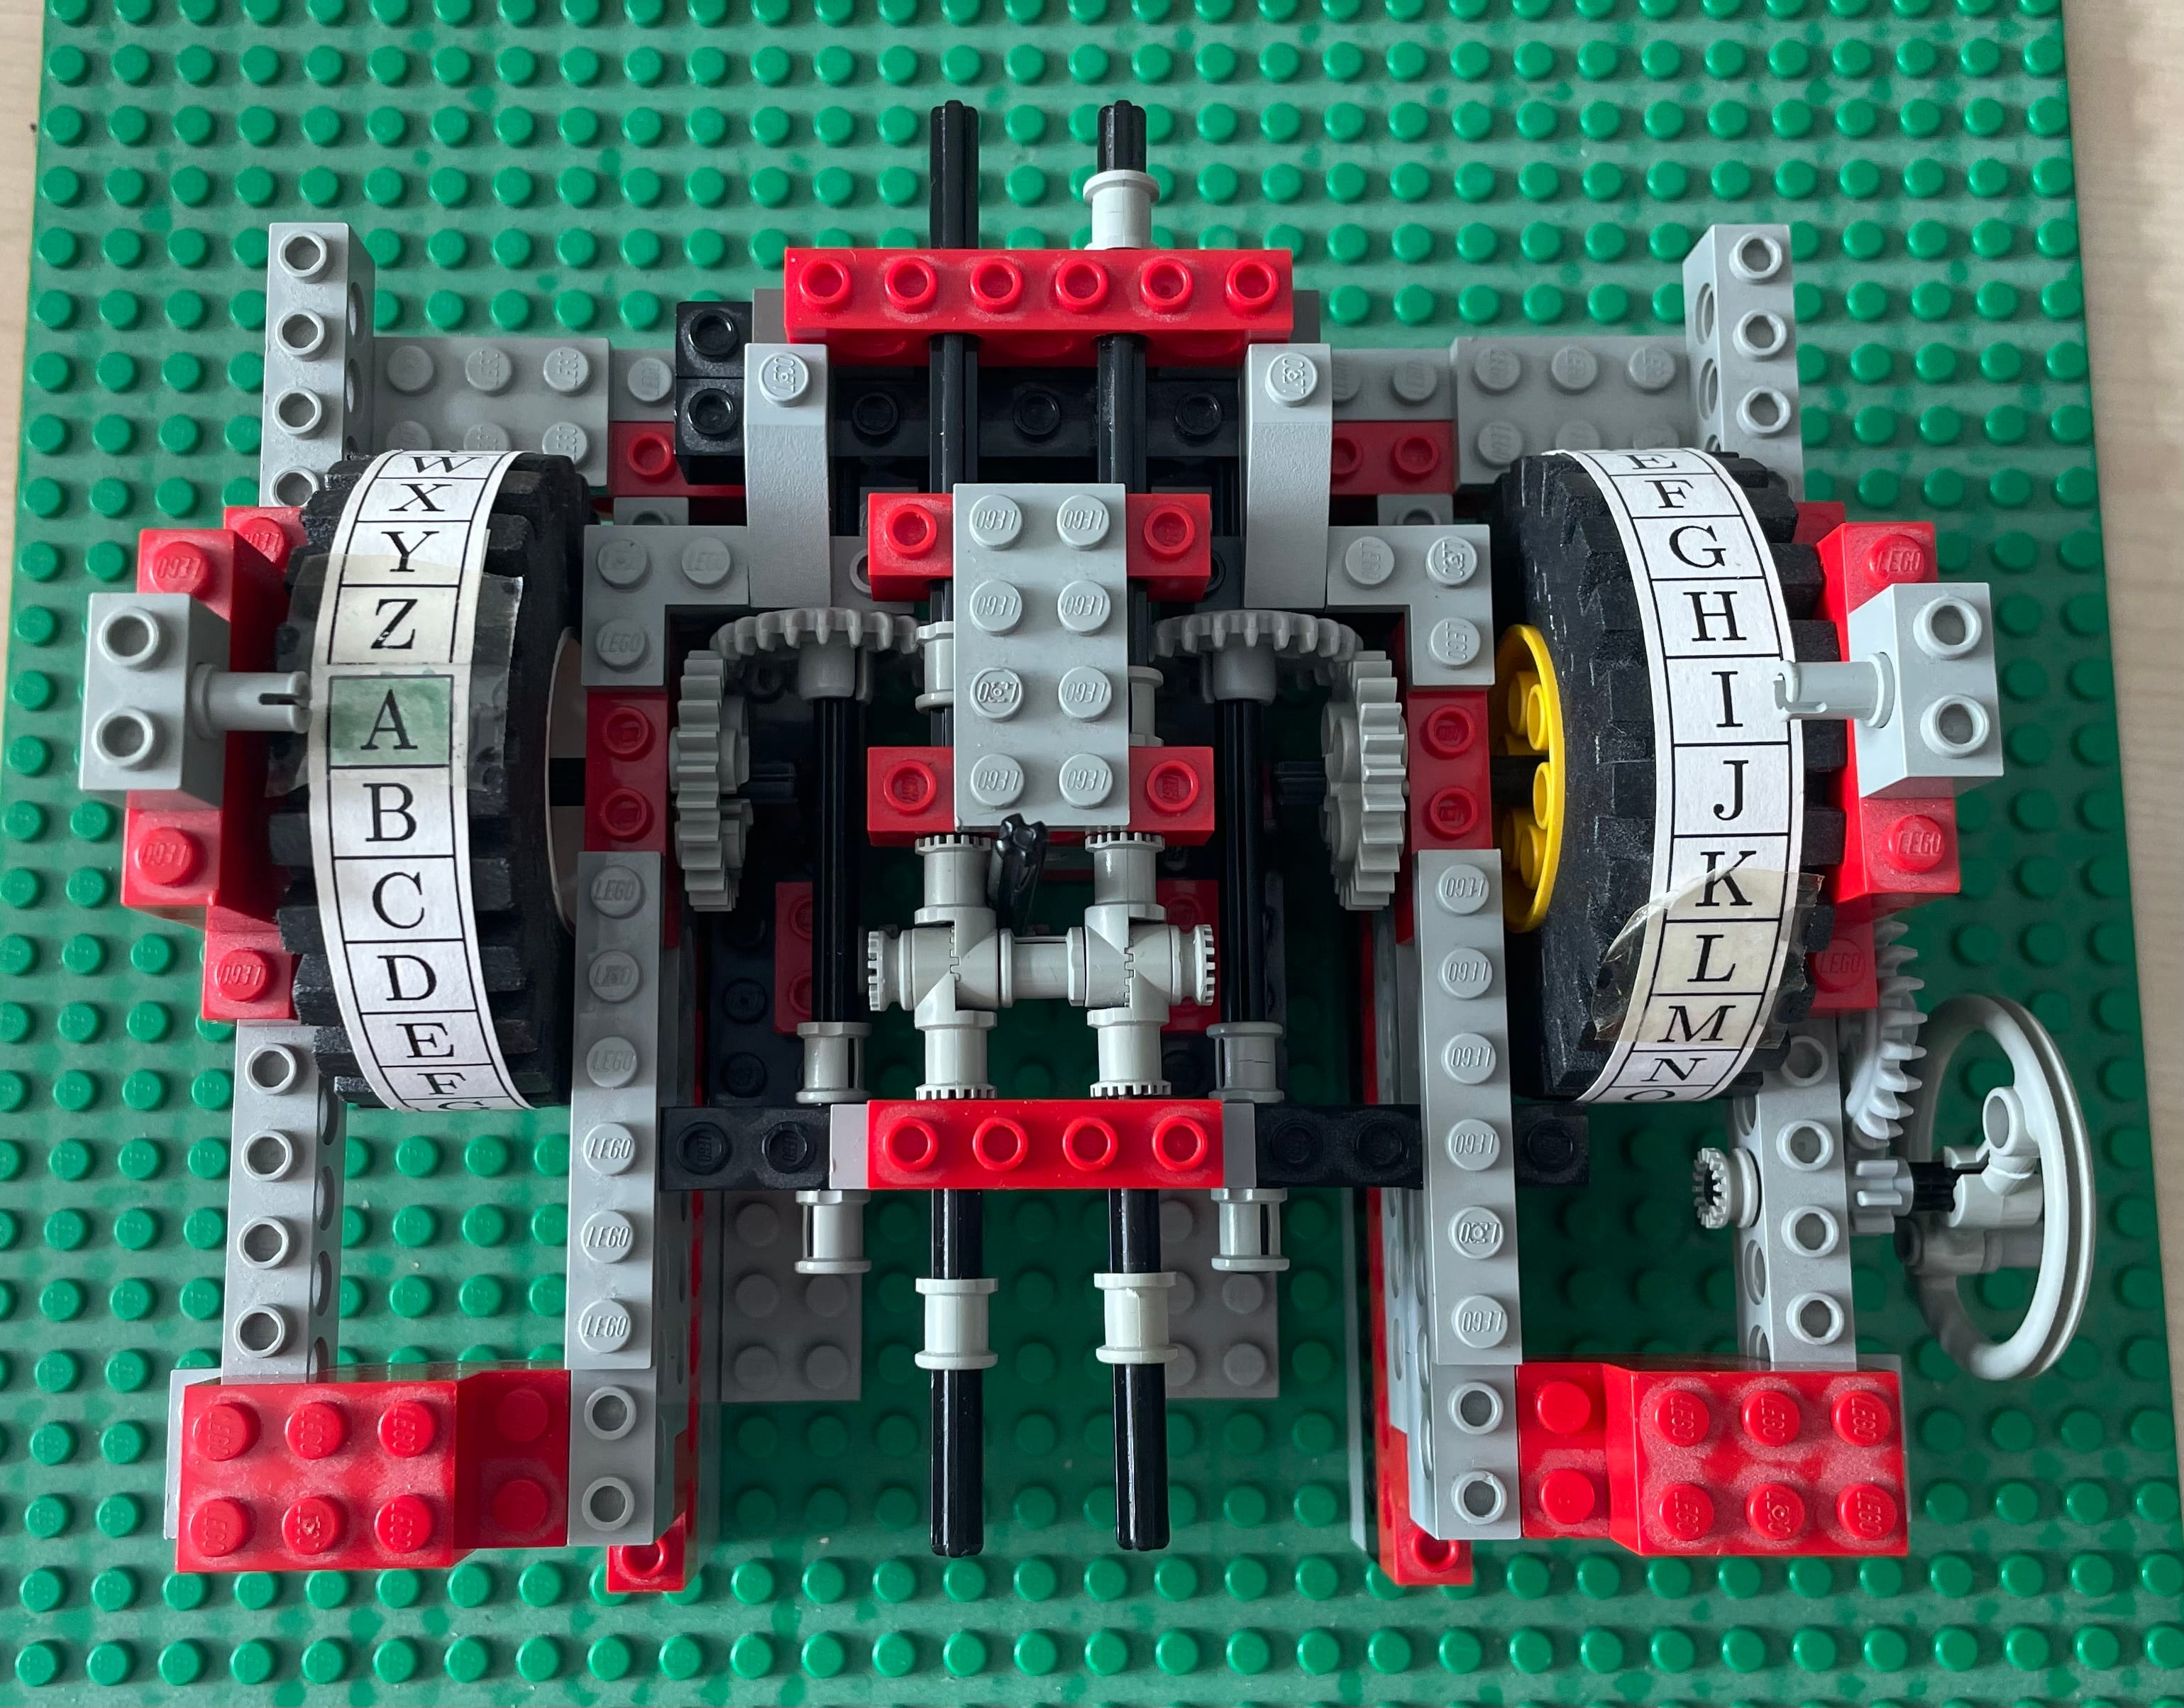
\includegraphics[width=200pt]{./Bilder/Fertig_gleich.jpg}}
		\caption{Fertige Lego-Engima.}
	\end{minipage}
	\end{figure}
	
\end{document}
